\chapter{Methodology}
\label{c:methodology}

This chapter details the methodology adopted to develop and validate the proof-of-concept implementation for the
proposed model reporting paradigm.
It begins with an in-depth technical discussion of the approach taken,
followed by detailing how it was implemented,
and concludes with an explanation of the evaluation strategy used to assess the approach.

% Specifics to openCAESAR
Although the model reporting paradigm is proposed for all of \gls{mbse},
the implementation is scoped to the openCAESAR framework.
Hence, certain specifics of the approach are tailored to its nature,
see \Cref{s:particularsProofOfConcept}.

\section{Approach}

The following section will first detail the architecture,
afterwards the choices that determined its design are justified.
Lastly, the contributions of the approach are put forward.

\subsection{System Architecture}
\label{s:sysArch}

Before delving into the specifics of the architecture,
a high-level overview of the pipeline and its constituents is given.
Each component is then explored in detail,
with a running example introduced at the start of each section when applicable,
to illustrate its functionality in context.
The running example is rooted in a specific domain, namely \glsentryfull{orkg}, 
that treats scientific papers and authors.
Further details about \gls{orkg} are provided in \Cref{s:knowledge_graph_and_benchmark},
since it will also be used for the experimental evaluation, see \Cref{s:experiments}.
The question starting the running example is given by \Cref{lst:runningExampleQuestion}.

\begin{listing}[!ht]

	\mint{text}{Question:}
	\mint{text}{Provide a list of papers that have utilized the Depth DDPPO model and include the links to their code?}

	\caption{Running example: question.}
	\label{lst:runningExampleQuestion}
\end{listing}

\subsubsection{High Level Overview}

Circling back to the model reporting paradigm (\Cref{fig:implementationExample}),
three aspects are essential:
the notebook environment, the agent that interacts with the system,
and finally the bridge between the two.
This section details how all three were implemented in practice as
a Jupyter Notebook, a \gls{kgqa} pipeline and a Python package.

\paragraph{Notebook Environment}

Jupyter was selected as the notebook environment, given its ubiquity,
and the existence of similar \gls{ai} extensions to the platform.\footnote{
	Jupyter AI is an example of such an \gls{ai} extension, available at \url{https://github.com/jupyterlab/jupyter-ai}.
}
Besides serving as the editing environment, it also renders the returned results from the pipeline and is the source
of the final report.

% Mid level of abstraction
\paragraph{Pipeline}

The \gls{kgqa} pipeline was introduced in \Cref{s:implementation} as part of the proof-of-concept implementation,
see \Cref{fig:pocImplementation}.
A more detailed view of the text-to-\gls{sparql} component of the pipeline is illustrated in \Cref{fig:textToSparql},
which includes its subcomponents: a domain expert, a translator, and a linker.

\input{src/schematics/tikzstyles}

\begin{tikzpicture}[auto, scale=1.0]

\node (nlq) {\small Question};

\node[block, below=0.5cm of nlq] (squall) {\small Text-to-prelinked-SQUALL};
\node[block, below=0.5cm of squall] (sparql) {\small SQUALL-to-SPARQL};
\node[block, below=0.5cm of sparql] (link) {\small Linking};

\node[below=0.5cm of link] (link_out) {\small SPARQL};

\path[arrow] (nlq.south) -- (squall.north);
\path[arrow] (squall.south) -- node[midway, right] {\small 1} (sparql.north);
\path[arrow] (sparql.south) -- node[midway, right] {\small 2} (link.north);
\path[arrow] (link.south) -- node[midway, right] {\small 3} (link_out.north);

\end{tikzpicture}


Common approaches for the text-to-\gls{sparql} task frequently train an \gls{llm} on a sizeable high-quality dataset
consisting of question-\gls{sparql} pairs for the target domain.
Due to the specialized domains in \gls{mbse} and associated data scarcity, this is not realistically feasible.
Hence, the text-to-\gls{sparql} task is deconstructed in three of the five stated components: the domain expert, translator and linker components;
combined they are responsible for the task.
The domain expert is tailored to a specialized domain and can generate a query for an input question.
Instead of \gls{sparql}, the target language is \gls{squall}, which was introduced in \Cref{s:cnl}.  
For further justifications behind choosing this \gls{cnl}, refer to \Cref{s:SQUALLOverSPARQL}.
However, translation from \gls{squall} to \gls{sparql} is needed in order to query the system.
Furthermore, the domain expert's output does not contain explicit identifiers from the target domain,
relying on textual placeholders instead.
For example, where a normal query targeted at Wikidata might contain an identifier such as \mintinline{sparql}{wd:Q30642},
output of the domain expert would contain the following placeholder: \mintinline{text}{natural language processing}.
The linker component stands in for associating the placeholders to identifiers.
To recap, for any given question the domain expert generates equivalent \gls{squall} containing placeholders,
which is mapped to \gls{sparql} by the translator and finally associated to the target \gls{kg} by the linker,
see \Cref{fig:textToSparql}.
Hereafter, assuming semantic correctness, a query can be executed, and its results handled by the ultimate component.
Practically, in case a user chose for visualization the execution of the query is also handled by the visualization engine.
For tabular results only execution is necessary.
A natural language answer can be generated by prompting a \gls{pllm} to answer the input question given the query results.
To that end, the prompt is constructed from the input question, task description and limited query results based
on context window size.

The order of the translator and linker as well as the choice of using placeholders instead of identifiers
are explained in \Cref{s:order_translator_and_linker} and \Cref{s:why_placeholders}, respectively.

% Low level of abstraction
\paragraph{Domain Expert}

The domain expert’s role involves generating \gls{squall} queries that are specifically ``tailored'' to the target domain.
While many syntactically correct queries can be equivalent in some sense for a given query language and input question,
only those appropriately tailored to the target domain would be relevant, matching the structure of the target \gls{kg},
i.e., those queries that are semantically correct.
This is essential in order to have executable queries.
The core issue of the data-scarce scenario then becomes clear:
it is not possible to reuse a model-centric and data-driven approach tailored to an original domain
for a distinct new one without any alterations, generated queries would not be semantically correct.
The idea presented here to overcome this problem is a type of transfer learning where knowledge gained in the 
original domain is transferred to the target domain.
Achieving this tailoring to the target domain and overcoming the data-scarce scenario.
An \gls{llm} is trained in the original domain on text-to-\gls{squall} task,
from this point onward it is referred to as the ``\gls{squall} expert''.
The knowledge it gained is leveraged by incorporating it in a \gls{rag} model as the generator component.
This final model is named the domain expert, since it has access to non-parametric domain information.
The training regime can be described as sequential training \cite{fanSurveyRAGMeeting2024},
where the generator is first fine-tuned on a specific task,
then frozen for further training of the \gls{rag} model.
Freezing the \gls{squall} expert means preventing catastrophic forgetting of its knowledge.
The retriever approach is straightforward,
and post-retrieval processing \cite{gaoRetrievalAugmentedGenerationLarge2024} is static,
neither require training.
The augmentation process does retrieval only once, supplying structured data to the generator component
(\gls{squall} expert) \cite{gaoRetrievalAugmentedGenerationLarge2024}.
Currently, only the augmentation process stands in for adaption to the target domain during the second phase of 
sequential training.
In conclusion, the domain expert is a \gls{rag} architecture consisting of
a generator separately fine-tuned during an initial training phase
--- dubbed the ``\gls{squall} expert''
--- a static retriever with post-retrieval processing,
and an augmentation method optimized during the second round of sequential training,
see \Cref{fig:domain_expert}.

\begin{figure}[ht!]
	\centering
	\begin{tikzpicture}[scale=1.0, transform shape]
		\tikzset{node distance = 30pt and 30pt}

		\node[draw, ellipse, minimum height=30pt, minimum width=90pt] (Q) {Question};
		\node[right=of Q, minimum height=30pt, minimum width=90pt, label={above:KG}] (KG) {};
		\node (kg) at (KG.center) {\includesvg[height=30pt]{kg.svg}};
		\node[draw, below=50pt of KG, minimum height=30pt, minimum width=90pt] (I) {Indexing};

		\node[below=50pt of Q, minimum height=30pt, minimum width=90pt] (n1) {};
		\node[below=of n1, minimum height=30pt, minimum width=90pt] (n2) {};
		%\node[below=of I, minimum height=30pt, minimum width=90pt] (n3) {};
		%\node[draw,fill=white, fit=(n2) (n3), inner sep=0pt] (R) {};
		%\node[fill=white] (n5) at (R.center) {Retrieval};

		\node[draw, text centered, below=of I, minimum height=30pt, minimum width=90pt, text width=80pt] (R) {Retrieval};

		\node[below=of n2, minimum height=30pt, minimum width=90pt] (n6) {};
		\node[below=of n6, minimum height=30pt, minimum width=90pt] (n10) {};
		\node[below=of n10, minimum height=30pt, minimum width=90pt] (n11) {};
		\node[draw, below=of n11, minimum height=30pt, minimum width=90pt, fill=blue!20] (E) {Text Embedder};

		\node[draw, text centered, below=of R, minimum height=30pt, minimum width=90pt, text width=80pt] (PR) {Post-Retrieval};
		\node[draw, below=of PR, minimum height=30pt, minimum width=90pt, fill=red!20] (GE) {Graph Embedder};
		\node[draw, below=of GE, minimum height=30pt, minimum width=90pt, fill=red!20] (P) {Projector};

		\node[below=of E, minimum height=30pt, minimum width=90pt] (n7) {};
		\node[below=of P, minimum height=30pt, minimum width=90pt] (n8) {};
		\node[draw, below=of n8, minimum height=30pt, minimum width=90pt] (n12) {};
		\node[draw, fit=(n7) (n12), inner sep=0pt, fill=blue!20] (SAL) {};
		\node (sal) at (SAL.center) {Self-Attention Layers};

		\node[draw, ellipse, below=50pt of SAL, minimum height=30pt, minimum width=90pt] (O) {\glsentryshort{squall}};

		\draw[->] (Q) -- (E) {};
		\draw[->] (Q) |- (R) node[midway, fill=white] {1};
		%\draw[->] (n2) -- (E) node[midway, fill=white] {1};
		\draw[->] (E) -- (n7) node[midway, fill=white] {2};
		\draw[->] (KG) -- (I) {};
		\draw[->] (I) -- (R) node[midway, fill=white] {3};
		\draw[->] (R) -- (PR) node[midway, fill=white] {4};
		\draw[->] (PR) -- (GE) node[midway, fill=white] {5};
		\draw[->] (GE) -- (P) node[midway, fill=white] {6};
		\draw[->] (P) -- (n12) node[midway, fill=white] {7};
		\draw[->] (SAL) -- (O) {};

		\node[draw, fit=(E) (SAL), densely dotted, very thin, inner sep=5pt,
		label={[xshift=20pt, yshift=0pt]below left:\scriptsize \glsentryshort{squall} Expert (Generator)}] (SE) {};

		\node[draw, fit=(GE) (P), densely dotted, very thin, inner sep=5pt,
		label={[xshift=45pt, yshift=0pt]above left:\scriptsize Augmentation}] (AP) {};

		\begin{scope}[on background layer]
			\node[draw, fit=(I) (R) (PR) (AP), dash dot dot, very thin, inner sep=5pt,
			label={[yshift=-120pt, rotate=90]above left:\scriptsize Learned Soft Graph Prompt}] (LSGP) {};
		\end{scope}

		\node[draw, fit=(LSGP) (R) (SE), dashed, very thin, inner sep=15pt,
		label={[xshift=-100pt, yshift=0pt]above:\footnotesize Domain Expert}] (DE) {};

		% Legend using a matrix
		\matrix [fill=white, matrix of nodes, nodes={anchor=west}, column sep=0.5cm, row sep=0.2cm, right=of DE, font=\small] {
			1 & Question \\
			2 & Text tokens \\
			3 & Vertex and edge embeddings \\
			4 & Top-$k$ vertices and edges \\
			5 & Minimum connected subgraph \\
			6 & Graph embedding \\
			7 & Aligned graph token \\
			\node[align=left, circle, minimum height=5pt, minimum width=5pt, fill=blue!20] (First) {};
				& \node[align=left, text width=145pt] {First phase of sequential training:\\
					{\footnotesize The \glsentryshort{squall} expert is independently fine-tuned on the source domain.}
				}; \\
			\node[align=left, circle, minimum height=5pt, minimum width=5pt, fill=red!20] (Second) {};
				& \node[align=left, text width=145pt] {Second phase of sequential training:\\
					{\footnotesize The domain expert is trained on the target domain, only the augmentation process is tuned,
					the \glsentryshort{squall} expert remains frozen, and other components are static.}
				}; \\
		};


	\end{tikzpicture}
	\caption{Domain Expert.}
	\label{fig:domain_expert}
\end{figure}



\paragraph{Retrieval}

Static retrieval consist of finding the most appropriate vertices and edges of the \gls{kg} for a given question.
This is achieved through textual similarity between the question and \mintinline{sparql}{rdfs:label} of all vertices and edges.

\paragraph{Post-Retrieval Processing}

The retrieved information is used to find a question-relevant subgraph of the \gls{kg} (structured data).
First, the sets of appropriate vertices and edges are ranked based on the similarity score.
Then they are assigned a certain value, called prize, based on their rank.
Using the \gls{pcst} algorithm,
a connected subgraph of the \gls{kg} can be found that both maximizes the total prize,
while minimizing the total cost, which is related to its size.

\paragraph{Augmentation}

The augmentation process first embeds the graph resulting from post-retrieval processing into an embedding
followed by ``aligning'' it with the \gls{squall} expert, i.e., with the \gls{llm}'s text embedding space.

\paragraph{SQUALL Expert}
\label{s:squallExpert}

The augmentation process employed to support the \gls{squall} expert is atypical in its approach,
as it integrates with the intermediate layers of the model \cite{fanSurveyRAGMeeting2024}.
Specifically, retrieved data is utilized at the self-attention layers of the \gls{llm},
rather than at the input or output layers
(i.e., input-layer or output-layer integration, respectively) \cite{gaoRetrievalAugmentedGenerationLarge2024}.
% Example
As a concrete example, a graph resulting from post-retrieval processing can contain over \num{300000} tokens.
%
Furthermore, since embeddings instead of text are used, other techniques can be leveraged.
If input-layer integration was used, the question-relevant graph would need to be linearized,
e.g., using a tabular overview of its vertices and edges.
The idea to use intermediate-layer integration for graph learning tasks was recently put forward \cite{liuCanWeSoft2024}.
This leads to an approach dubbed soft graph prompting,
and has the advantage of having the ability to pass the retrieved graph
through a graph embedder and directly using that advantageous representation instead of a linearized representation,
which results in loss of the graph's topological information.
The hypothesis that soft graph prompting can aid \gls{llm} generation for graph learning tasks was further investigated
by \cite{heGRetrieverRetrievalAugmentedGeneration2024} on a \gls{qa} task.
%
A notable distinction between the prior works \cite{liuCanWeSoft2024, heGRetrieverRetrievalAugmentedGeneration2024}
and the approach presented here lies in the following:
the \gls{squall} expert undergoing soft graph prompting has already been fine-tuned for a specific task.
%
It is important to note that the level of access required for implementing soft graph prompting is unavailable for most
\glspl{llm} accessed via inference \glspl{api} \cite{fanSurveyRAGMeeting2024}.
These models operate largely as black boxes:
users provide input and receive output, but the internal processes remain inaccessible.
Prominent examples, such as ChatGPT, Gemini, and Claude, do not support this type of prompting.

% Recap: Proof-of-Concept --> OML ontolgies --> KG --> RDF graph
\subsubsection{Particulars of the Proof-of-Concept}
\label{s:particularsProofOfConcept}

First, a short note on the particulars of the proof-of-concept.
As briefly touched upon in \Cref{s:systemDesign}, the proof-of-concept implementation of the model reporting paradigm
is tailored to the openCAESAR framework, a representative \gls{mbse} approach.
Like other \gls{mbse} approaches, the openCAESAR framework uses models to represent systems.
Distinct to openCAESAR, these models are defined using the \glsentrylong{oml},
a formal language inspired by \gls{owl2} and \gls{swrl}.

Looking again at Kepler16b,
an example of how a relation between its missions and their objectives could be modeled in \gls{oml}
is given by \Cref{lst:kepler16bVocabularyModel}.

\begin{listing}[!ht]
	\inputminted{text}{src/listings/kepler16b-vocabulary-model.oml}
	\caption{Kepler16b vocabulary model excerpt \cite{elaasarOpenCAESARBalancingAgility2023}.}
	\label{lst:kepler16bVocabularyModel}
\end{listing}

Like \gls{owl2}, \gls{oml} is used for authoring ontologies, but it is specifically tailored for \gls{se}.
% Ontology
An ontology is essentially a formal representation of knowledge about some domain, in this context a system.
% Implications ontology use
It is through \gls{oml} that openCAESAR introduces the ontological approach to \gls{mbse}.
This has many benefits for model authoring, e.g., enabling the use of a logical reasoner
that can check whether there are any logical contradictions present in the \gls{oml} model
\cite{elaasarOpenCAESARBalancingAgility2023}.

% Model authoring not the same as information retrieval
Answering questions or retrieving information about the model necessitates a different method: querying.
\gls{oml} constructs (such as \mintinline{text}{relation}) can be translated into patterns represented within subsets of
\gls{owl2} and \gls{swrl}.
Consequently, \gls{oml} ontologies can effectively be converted into \gls{owl} ontologies.

% Endpoints
Various tools can be used to query \gls{owl} ontologies in \gls{sparql} such as the \gls{owl} ontology editor
Protégé.
Alternatively, a so-called \gls{sparql} endpoint can be set up using platforms such as Apache Jena,
which only take the ontology and then allow users to query it using \gls{sparql}.

% RDF
Regardless of the approach chosen,
the ontology is typically stored in the \gls{rdf} format (discussed further below).
Internally, what is queried against is not a set of textual documents wherein the ontology is defined,
but rather a graph constructed from the \gls{rdf} format, i.e., the \gls{rdf} graph.

% OML --> OWL --> RDF
Thus, after model authoring the openCAESAR framework makes the model queryable
by mapping it to an \gls{owl} ontology and subsequently setting up a \gls{sparql} endpoint.
Note that it is necessary to repeat the process if the model is changed in order for the endpoint to be up-to-date.

% KG
Although in this proof-of-concept a model is ultimately made queryable through an \gls{rdf} graph,
this is just one type of graph data format and alternatives exist.
Neo4j, for example, uses property graphs instead of \gls{rdf} graphs.
Generally, this concept of using a graph of data to represent knowledge is called a \glsentryfull{kg}
\cite{hoganKnowledgeGraphs2022}.

\paragraph{Ontologies and Statements in Knowledge Bases}

The statements in any \gls{kb}/\gls{kg} can be categorized as either belonging to its \gls{tbox} or \gls{abox}.
The \gls{tbox} contains statements describing the domain of interest,
while the \gls{abox} contains ground statements, i.e., facts associated with, and compliant to, the \gls{tbox}.
For example, in the Kepler16b context, a \gls{tbox} statement might be, 
\mintinline[breaklines]{text}{"Every objective is pursued by a mission,"}
while a corresponding \gls{abox} statement could be,
\mintinline[breaklines]{text}{"The Lander Mission is a mission."}
%
If, for example, the \gls{tbox} statements are related with object-oriented classes,
the \gls{abox} statements would be instances of those classes.
%
Given the above highlighted relation between an ontology and a \gls{kb},
this distinction can also be made in the ontology,
both \gls{owl} and \gls{oml} ontologies do this.
However, the distinction is not set in stone, different ontologies categorize differently.
%
In openCAESAR,
the \gls{tbox} and \gls{abox} are referred to as the vocabulary and description models,
and they are similar to \gls{owl}'s \gls{tbox} and \gls{abox},
respectively \cite{elaasarOpenCAESARBalancingAgility2023}.
%
The Kepler16b system design example of \Cref{lst:kepler16bDescriptionModel} showed a part of the description model,
see \Cref{lst:kepler16bVocabularyModel} for its related vocabulary model.

\subsubsection{Formalization}

% Intro
The formalization presented in this section establishes the foundation for the subsequent discussions.
As outlined in the introduction,
the proposed approach is specifically tailored to models that can be represented as \glspl{kg},
implemented as \gls{rdf} graphs.
The graph formalisms introduced here are particularly relevant to \Cref{s:postRetrieval},
which describes an algorithm designed to identify subgraphs relevant to specific questions.
The aim is to use standardized terminology, fostering consistency and clarity across the methodology.
Established concepts from the literature are leveraged to ensure alignment with existing conventions 
and to improve comprehensibility.
In particular, the definitions provided by \cite{zouGraphBasedRDFData2017}
and the notations introduced by \cite{thakkarIntegratedGraphAlgebra2019} are adopted.

% Next
First, the \gls{rdf} format is first introduced in order to gain insight on how a model in openCAESAR is actually
represented when it is queried, which is crucial for retrieval and post-retrieval,
see \Cref{s:retrieval} and \Cref{s:postRetrieval}, respectively.
Basic concepts from the \gls{rdf} framework are introduced, for example,
\glspl{uri}, \glspl{bnode} and literals, which are important for linking (\Cref{s:linking}).

% Introduce RDF framework
Beginning then with the \gls{rdf} framework which represents data as semantic triples,
such as \emph{"model reporting is flexible."} 
Each triple adheres to the structure \emph{"subject predicate object"}, where:  
\begin{itemize}
	\item \textbf{Subject} identifies the resource being described (\emph{model reporting}).
    \item \textbf{Predicate} specifies the property or relationship (\emph{is}).
    \item \textbf{Object} provides the value or linked resource (\emph{flexible}).
\end{itemize}

These triples collectively form a graph, as illustrated in \Cref{fig:rdfGraph}.\footnote{
	Example from a W3C working draft about RDF available at
	\url{https://www.w3.org/2001/sw/RDFCore/TR/WD-rdf-concepts-20030117}.
}

\begin{figure}[h!]
	\centering
	\begin{tikzpicture}[
    node/.style={draw, rounded corners, align=center, minimum width=2.5cm, minimum height=1cm},
    edge/.style={->, thick},
    scale=0.6, transform shape
]

% Nodes
\node[node, label=above:{$v_1$}] (v1) {\small \texttt{http://www.example.org/staffid/85740}};
\node[node, below=2cm of v1, label=below:{$v_2$}] (v2) {};

\node[node,  below left=2cm and 3cm of v2, label=below:{$v_3$}] (v3) {'Bedford'};
\node[node,  below left=5cm and 0cm of v2, label=below:{$v_4$}] (v4) {'1501 Grant Avenue'};
\node[node,  below right=5cm and 0cm of v2, label=below:{$v_5$}] (v5) {'01730'};
\node[node,  below right=2cm and 3cm of v2, label=below:{$v_6$}] (v6) {'Massachusetts'};

% Edges
\draw[edge] (v1) -- node[midway, left] {\small \texttt{http://www.example.org/city}} (v2);
\draw[edge] (v2) -- node[pos=0.85, left] {\small \texttt{http://www.example.org/address}} (v4);
\draw[edge] (v2) -- node[midway, left=0.2cm] {\small \texttt{http://www.example.org/street}} (v3);
\draw[edge] (v2) -- node[pos=0.85, right] {\small \texttt{http://www.example.org/postalCode}} (v5);
\draw[edge] (v2) -- node[midway, right=0.2cm] {\small \texttt{http://www.example.org/state}} (v6);

\end{tikzpicture}

	\caption{
		Example \glsentryshort{rdf} graph, representing a staff member and relationships to its associated properties
		such as city, address, street, postal code, and state.
	}
	\label{fig:rdfGraph}
\end{figure}

The figure highlights three fundamental \gls{rdf} terms:  
\begin{itemize}
    \item \textbf{\gls{uri}}: A globally unique identifier representing a resource.
	 \item \textbf{\gls{bnode}}: An unnamed resource or existential variable.
    \item \textbf{Literal}: A value such as a string, number, or date.
\end{itemize}

In \gls{rdf}, resources can act as classes, which define categories or types;
entities, which are specific instances of those categories;
or properties, which describe relationships or attributes connecting entities or values.

Formally these notions can be defined as follows.

\begin{definition}
	\label{def:rdfDataset}
	An \textit{\gls{rdf} dataset } is a set $\mathscr{D}$ of triples
	$t = (\text{subject}, \text{property}, \text{object}) \in (I \cup B) \times I \times (I \cup B \cup L)$.\footnote{
		Triples are sequences of three elements.
	}
	The pairwise disjoint infinite sets $I$, $B$ and $L$ indicate \glspl{uri},
	\glsentryfullpl{bnode} (or vertices) and literals.

\end{definition}

Before querying an \gls{oml} ontology is mapped to an \gls{owl} ontology and stored in an \gls{rdf} dataset.

\begin{definition}
	An \textit{\gls{rdf} graph} is a graph $G = (V, L_V, E, L_E)$
	where 

	\begin{defitemize}

		\item 
			$V = V_c \cup V_e \cup V_b \cup V_l $ is a set of vertices consisting of all subjects and objects in the
			\gls{rdf} data, with $V_c$, $V_e$, $V_b$ and $V_l$ being the set of class, entity, blank and literal vertices,
			respectively.

		\item $L_V$ is a set of vertex labels, for a vertex $v \in V_c \cup V_e$, $v \in V_b$ and $v \in V_l$ 
			their labels correspond to \glspl{uri}, \mintinline{text}{NULL} values and literals, respectively.

		\item $E \subseteq V \times V $ is a set of directed edges, and

		\item $L_E$ is a set of edge labels, for an edge $e \in E$, its label is its property.

	\end{defitemize}

\end{definition}

Applying to the example graph (\Cref{fig:rdfGraph}) with vertices $V = V_c \cup V_e \cup V_b \cup V_l $: \\
$V_c = \emptyset, \quad V_e = \Set{ v_1 }, \quad V_b = \Set{ v_2 }, \text{and} \quad V_l = \Set{ v_3, v_4, v_5, v_6 }$.
	
Querying is done against the \gls{rdf} graph representation of an ontology,
though any user is naturally shielded from any graph-related concepts and technical details,
as these are abstracted away (see \Cref{s:particularsProofOfConcept}).

However, a foundational understanding of elementary graph theory is essential to clearly explain the proposed approach
in the sections that follow.
Therefore, these concepts are introduced upfront.
While the following formalizations might often be avoided,
they are considered to serve an important role in aligning with a theoretical framework that promotes academic rigor and,
crucially, ensures consistency. 
For instance, the domain expert could be introduced solely in terms of generated queries,
but this approach would not seamlessly align with the other components.
See, for example, the discussion of the post-retrieval component in \Cref{s:postRetrieval},
it outputs graphs.
However, since queries are inherently related to graphs, as will be elaborated upon,
structuring the domain expert's discussion around graphs ensures a cohesive and unified narrative.

\begin{definition}
	A \textit{subgraph} \( H \) of a graph \( G \) is defined as a graph such that:
	\[
		H = (V_H, E_H), \quad \text{ where } V_H \subseteq V \text{ and } E_H \subseteq E.
	\]
	In this notation, \( V_H \) and \( E_H \) represent the sets of vertices and edges of the subgraph \( H \), respectively.
\end{definition}

\begin{definition}
	Two vertices \( v \) and \( w \) in a graph \( G \) are said to be \textit{adjacent}
	if there is an edge connecting them:
	\[
		v \text{ and } w \text{ are adjacent} \iff (v, w) \in E \text{ or } (w, v) \in E.
	\]
\end{definition}

\begin{definition}
	A \textit{path} $p$ in a graph $G$ is a finite sequence of vertices:
	\[
		\begin{aligned}
									& p = \Set{ v_i }_{i=0}^n \in E^*, \quad n < \infty \\
			\text{s.t.} \quad & \forall i, j \in \Set{ 0, 1, \ldots, n }: i \neq j \land v_i \neq v_j 
						\implies v_i \text{ and } v_j \text{ are adjacent},
		\end{aligned}
	\]
	where $^*$ is the Kleene star operation.\footnote{
		The Kleene star operation $^*$ constructs the free monoid $E^* = \bigcup_{n=0}^{\infty} E^n$,
		where $E^0 = \Set{ \varepsilon }$ and $\varepsilon$ is the identity (or empty) element
		\cite{thakkarIntegratedGraphAlgebra2019}.
	}
\end{definition}

\begin{definition}
	A graph $G$ is said to be \textit{connected} when there exists a path in between every pair of its vertices joining 
	the pair:
	\[
		G \text{ is connected } \iff \forall v, w \in V, \; v \neq w, \; \exists \; p \in E^*: v, w \in p
	\]
\end{definition}

\paragraph{Connected Subgraphs}
Without delving further into graph theory, a shorthand notation can be introduced to represent all possible connected
subgraphs of a graph $G$ using the concept of the hyperspace graph of connected subgraphs $ \mathscr{C}(G) $,
which is defined for any connected graph \cite{likincsimonromeroUniquenessHyperspaceGraph2007, likincsimonromeroHyperspaceGraphConnected2005}.
Relevant here is that any connected subgraph $H$ of $G$ is an element of the vertex set of $\mathscr{C}(G)$
by definition:
\[
	V_{\mathscr{C}(G)} = \{ H; H \in \mathscr{C} \land H \subseteq G \},
\]
where $\mathscr{C}$ is the set of all connected graphs.

\paragraph{Vertex and Edge Similarity}

The similarity between a string and a vertex or edge of a graph $G$ is defined using an arbitrary encoder \gls{lm} $\lambda$:
\[
	\lambda: \Sigma^* \rightarrow X
\]
where $\Sigma^*$ is the set of all strings over some alphabet $\Sigma$,
and $X$ is an arbitrary set, e.g., $\mathbb{R}^n$.
By a slight abuse of notation, vertices and edges can also be used as input to $\lambda$,
with the implicit assumption that with each vertex or edge a string can be associated.
In the case that $G$ is a \gls{kg}, that string is a vertex's or edge's metadata property \mintinline{sparql}{rdfs:label},
this attribute being the human-readable name of the resource.
A set of graph embeddings is referred to as an index $ \mathscr{I} $.
If all embeddings result from one graph $ G $, e.g., a \gls{kg},
the graph's index is defined as follows:
\begin{align}
	\mathscr{I}_G &= \Set{ \lambda(x) \mid x \in V \cup E }.
	\label{eq:index}
\end{align}
A function $\sigma$ is used to assess the similarity between embeddings, denoted by $\sigma(x, y)$.
For convenience, this notation is also extended to allow strings, vertices, and edges as inputs,
with the understanding that the similarity function implicitly operates on their embeddings.
Specifically, define:
\begin{align}
	\sigma(s, x) \coloneqq \sigma(\lambda(s), \lambda(x)), 
	\quad s \in \Sigma^*, \; x \in V \cup E,
	\label{eq:similarityFunction}
\end{align}
The specific similarity function $\sigma$ used in the experiments is detailed in \Cref{s:settings_retrieval}.

\begin{definition}
	A \textit{\glsentryfull{bgp}} is defined as graph $Q = (V_Q, E_Q) \in \mathscr{C}$ s.t.:
	\begin{defitemize}

		\item 
			$V_Q \subseteq I \cup L \cup V_{\text{var}}$ is a set of vertices,
			with $I$, $L$ and $V_{\text{var}}$ being the of \glspl{uri}, literals and variables, respectively.

		\item 
			$E_Q \subseteq V_Q \times V_Q $ is a set of edges

		\item An edge in $E_Q$ either has an edge label in $I$, i.e., property, or is a variable.
		
	\end{defitemize}
\end{definition}

An example of a \gls{bgp} is illustrated by \Cref{fig:sparqlBGP}.

\begin{figure}[!ht]
	\centering

	\begin{subfigure}[t]{0.45\textwidth}
		\centering
		\vspace{0pt}
		\inputminted{sparql}{src/listings/bgp-pattern.sparql}
	\end{subfigure}
	\hfill
	\begin{subfigure}[t]{0.45\textwidth}
		\centering
		\vspace{0pt}
		\centering
		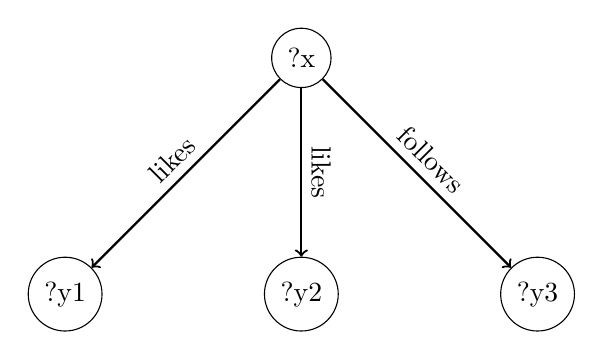
\begin{tikzpicture}[
    node distance=2cm and 3cm,
    node/.style={draw, circle, align=center},
    edge/.style={->, thick},
    slopedlabel/.style={midway, sloped, above, text=black},
]

% Nodes
\node[node] (x) at (0, 0) {?x};
\node[node] (y1) at (-3, -3) {?y1};
\node[node] (y2) at (0, -3) {?y2};
\node[node] (y3) at (3, -3) {?y3};

% Edges
\draw[edge] (x) -- node[slopedlabel] {likes} (y1);
\draw[edge] (x) -- node[slopedlabel] {likes} (y2);
\draw[edge] (x) -- node[slopedlabel] {follows} (y3);

\end{tikzpicture}

	\end{subfigure}

	\caption{Example of \glsentrylong{bgp} with a star shape \cite{schatzleS2RDFRDFQuerying2016}.}
	\label{fig:sparqlBGP}
\end{figure}

\glspl{bgp} are the starting point of \gls{sparql} queries which are used to inquire into \gls{rdf} graphs.
To formalize the entirety of the \gls{sparql} language \glspl{cgp} are needed, 
which are in essence \glspl{bgp} with additional operations including projections and unions,
e.g., the \mintinline{sparql}{FILTER} \cite{thakkarIntegratedGraphAlgebra2019}.
Hereafter, they are both mentioned as \glspl{gp}.

Presented here is the \glsentryfull{pgp}, a graph similar to the \glsentryfull{gp}.
However, it uses string literals, referred to as placeholders, instead of \glspl{uri}.  

The \gls{bgp} example shown in \Cref{fig:sparqlBGP} is in fact a \gls{pgp}, given that instead of \glspl{uri},
strings are used for the edges.
In contrast to the previous example of \Cref{fig:rdfGraph}.

\begin{definition}
	A \textit{\glsentryfull{pgp}} is defined as a graph $\hat{Q} = (V_{\hat{Q}}, E_{\hat{Q}}) \in \mathscr{C}$ s.t.:
	\begin{defitemize}
		\item 
			$V_{\hat{Q}} \subseteq P \cup L \cup V_{var}$ is a set of vertices,
			with $P$, $L$ and $V_{var}$ being the set of placeholders, literals and variables, respectively.,
		\item $E_{\hat{Q}} \subseteq V_{\hat{Q}} \times V_{\hat{Q}} $ is a set of edges,
		\item An edge in $E_{\hat{Q}}$ either has an edge label in $P$, i.e., property, or is a variable,
	\end{defitemize}
	where $P \subseteq \Sigma^*$.
\end{definition}

Reviewing the pipeline, a \gls{pgp} essentially serves as a precursor to a \gls{gp}:

\begin{enumerate}
	\item The domain expert generates a \gls{squall} expression containing placeholders,
		see \Cref{s:retrieval}--\Cref{s:generation}.
	\item Translation maps this expression to a \gls{pgp},
		i.e., a \gls{sparql} query where the placeholders have not yet been filled in with actual \glspl{uri},
		see \Cref{s:squallToSparql}.
	\item Linking maps the \gls{pgp} to a \gls{gp} in \gls{sparql},
		i.e., an executable query,
		see \Cref{s:linking}.
\end{enumerate}

See \Cref{fig:textToSparql} for the pipeline.\footnote{
	For clarity the schematics state \gls{sparql} instead of \gls{pgp}.
}

Finally, given a set of graphs $\mathscr{D}$,
the average number of vertices and edges is explicitly defined for clarity as follows:

\begin{align}
	\wideoverbar{V}_{\mathscr{D}} &= \frac{1}{|\mathscr{D}|}\sum_{G \in \mathscr{D}}|V_G| \label{eq:avgVertices} \\
	\wideoverbar{E}_{\mathscr{D}} &= \frac{1}{|\mathscr{D}|}\sum_{G \in \mathscr{D}}|E_G| \label{eq:avgEdges}.
\end{align}

\Cref{s:index} uses \Cref{eq:avgVertices} and \Cref{eq:avgEdges} to compare datasets containing graphs.

\subsubsection{Retrieval}
\label{s:retrieval}

Given a question targeted at a \gls{kg} = $(V, E)$,
retrieval consists of finding relevant information from its index $\mathscr{I}_{\text{\gls{kg}}}$,
see \Cref{fig:runningExampleRetrieval}.

\begin{figure}[!ht]
	\centering

	\mint{text}{Question:}
	\inputminted{text}{src/listings/running-example/question.txt}
	\mint{text}{}

	% Subfigure for the listing
	\begin{subfigure}[t]{0.26\textwidth}
		\vspace{0pt} % Ensures alignment at the top
		\inputminted{text}{src/listings/running-example/retrieval.txt}
		\caption{Retrieved vertices and edges.}
		\label{lst:runningExampleRetrievalLinearized}
	\end{subfigure}
	\hfill
	% Subfigure for the TikZ schematic
	\begin{subfigure}[t]{0.73\textwidth}
		\vspace{0pt} % Ensures alignment at the top
		\centering
		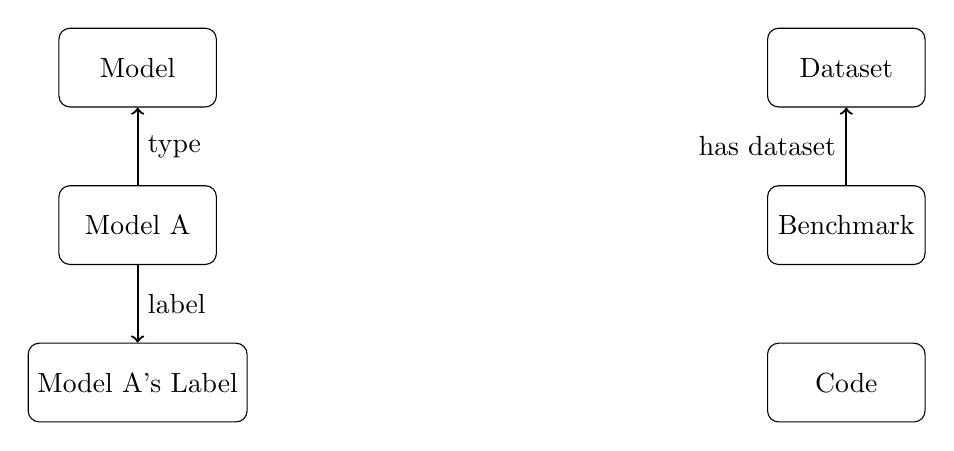
\begin{tikzpicture}[
	node/.style={draw, rounded corners, align=center, minimum width=2cm, minimum height=1cm},
	edge/.style={->, thick},
	scale=1, transform shape
]

% Left side nodes
\node[node] (modelA) at (-4.5, 0) {Model A};
\node[node] (model) at (-4.5, 2) {Model};
\node[node] (label) at (-4.5, -2) {Model A's Label};

% Right side nodes
\node[node] (benchmark) at (4.5, 0) {Benchmark};
\node[node] (dataset) at (4.5, 2) {Dataset};
\node[node] (code) at (4.5, -2) {Code};

% Edges
\draw[edge] (benchmark) -- node[midway, left] {has dataset} (dataset);
\draw[edge] (modelA) -- node[midway, right] {type} (model);
\draw[edge] (modelA) -- node[midway, right] {label} (label);

\end{tikzpicture}

		\caption{Graph representation.}
		\label{fig:runningExampleRetrievalGraph}
	\end{subfigure}

	\caption{Running example: retrieval.}
	\label{fig:runningExampleRetrieval}
\end{figure}

As stated, $\mathscr{I}_{\text{\gls{kg}}}$ is created by encoding all its vertices and edges using an \gls{lm}.
The subset of $k$ most similar vertices and edges for a given string $s$ is defined as:
\begin{align}
	&V_{s, k} = \arg \text{top}\,k _ { \, v \in V } \, \sigma(s, v), \label{eq:topkVertices} \\
	&E_{s, k} = \arg \text{top}\,k _ { \, e \in E } \, \sigma(s, e), \label{eq:topkEdges}
\end{align}
respectively, where $\arg \text{top}\,k _ { \, x \in X } \, f(x)$
essentially returns the $k$ elements from the set $ X $ that maximize the function $ f $ stated as its argument.
The similarity function $ \sigma $ was defined in \Cref{eq:similarityFunction}.
For an input strings $s \in \Sigma^*$,
the relevant information is defined as the subsets \( V_{s, k} \subseteq V \) and \( E_{s, k} \subseteq E \).

\paragraph{Nature of the Index}
\label{s:index}

The process of indexing
--- i.e., creating a set of graph embeddings $ \mathscr{I} $ (see \Cref{eq:index})
--- and retrieval differs significantly from the implementation in \cite{heGRetrieverRetrievalAugmentedGeneration2024}.
In their approach, a specific graph $H$ is associated with each question,
resulting in multiple graph indices $ \mathscr{I}_{H} $ rather than a unified index.
This design allows for retrieval within smaller, question-specific indices,
simplifying the search process compared to a comprehensive combined index.
However, the use of question-specific graphs assumes preprocessing steps if the starting point is a \gls{kg}.
%
In contrast, this thesis employs a single \gls{kg} as the foundation for all questions,
requiring retrieval from one unified, large-scale index $ \mathscr{I}_{\text{\gls{kg}}} $.
This approach leads to a significant disparity in graph sizes used as input for the \gls{pcst} algorithm.
Moreover, the \glspl{kg} used in \gls{mbse} are generally much larger than the graphs analyzed in
\cite{heGRetrieverRetrievalAugmentedGeneration2024} (see \Cref{s:size_kgb}).
Of the three datasets utilized in the original work, only WebQSP includes an underlying \gls{kg}.

The datasets used in \cite{heGRetrieverRetrievalAugmentedGeneration2024} are summarized as follows:

\begin{itemize}
	\item \textbf{ExplaGraphs} \cite{sahaExplaGraphsExplanationGraph2021}:
		Explanatory graphs, supporting and countering arguments are generated given a belief and an argument.
	\item \textbf{SceneGraphs} \cite{hudsonGQANewDataset2019}:
		Questions are generated from a scene graph structure.
	\item \textbf{WebQSP} \cite{yihValueSemanticParse2016}:
		Questions with subgraphs extracted from Freebase
		by extracting all triples that include entities related to the question within the maximum reasoning hops specified in WebQSP
		\cite{luoReasoningGraphsFaithful2024}.
\end{itemize}

For a detailed comparison of the datasets and their associated \glspl{kg},
refer to \Cref{table:comparisonDatasetsSamples} and \Cref{table:comparisonDatasetsKnowledgeGraphs}, respectively.

\begin{table*}[h]
	\centering

	\begin{tabular}{l|SSSS|r}

		\textbf{Dataset}
		& \textbf{\# Questions} & \textbf{\# Graphs} & \textbf{Average \# Vertices} & \textbf{Average \# Edges} & \textbf{Source} \\

		\hline
		
		\textbf{ExplaGraphs} & 2766  & 2766  & 5       & 4    & \cite{heGRetrieverRetrievalAugmentedGeneration2024} \\
		\textbf{SceneGraphs} & 10000 & 10000 & 19      & 68   & \cite{heGRetrieverRetrievalAugmentedGeneration2024} \\
		\textbf{WebQSP}      & 4737  & 4737  & 1371    & 4252 & \cite{heGRetrieverRetrievalAugmentedGeneration2024, luoReasoningGraphsFaithful2024} \\
		\textbf{SciQA}       & 2565  & 1     & 180184  & 6888 & \cite{auerSciQAScientificQuestion2023, auerSciQABenchmarkDataset2023} \\

	\end{tabular}

	\caption{
		Summary of datasets with key statistics including the number of questions, graphs, vertices, edges, and their sources.
	}

	\label{table:comparisonDatasetsSamples}
\end{table*}

\begin{table*}[h]
	\centering

	\begin{tabular}{l|rrrr|r}

		\textbf{Dataset}
		& \textbf{\glsentrylong{kg}} & \textbf{\# Triples} & \textbf{\# Vertices} & \textbf{\# Edges} & \textbf{Source} \\

		\hline
		
		\textbf{ExplaGraphs} & N/A         & N/A           & N/A           & N/A        & \cite{heGRetrieverRetrievalAugmentedGeneration2024} \\
		\textbf{SceneGraphs} & N/A         & N/A           & N/A           & N/A        & \cite{heGRetrieverRetrievalAugmentedGeneration2024} \\
		\textbf{WebQSP}      & Freebase    & 126M          & 88M           & 20K        & \cite{heGRetrieverRetrievalAugmentedGeneration2024, luoReasoningGraphsFaithful2024} \\
		\textbf{SciQA}       & \gls{orkg}  & \num{1133217} & \num{180184}  & \num{6888} & \cite{auerSciQAScientificQuestion2023, auerSciQABenchmarkDataset2023} \\

	\end{tabular}

	\caption{
		Overview of datasets and their associated (\glsentrylongpl{kg}),
		including triples, vertices, edges, and source references.
		\glsentryshort{orkg} version: February 14, 2023.
	}

	\label{table:comparisonDatasetsKnowledgeGraphs}
\end{table*}


\subsubsection{Post-Retrieval}
\label{s:postRetrieval}
%\TODO{Review ranking functions}

After retrieval, one set of vertices and one set of edges are obtained.
Together they do not necessarily form a connected subgraph.  
Crucial vertices and edges required to construct a semantically correct query,  
including triples that may not be easily inferable from the question, could also be absent.  
These challenges are addressed through post-retrieval processing,  
which produces a connected subgraph ideally encompassing all necessary triples.  
Refer to \Cref{fig:runningExamplePostRetrieval},  
which represents the post-processed version of \Cref{fig:runningExampleRetrieval}.  
It includes those additional vertices and edges that may not be as straightforward to infer as others, 
yet are essential for accurately parsing the question, e.g., \mintinline{text}{content}.

\begin{figure}[!ht]
	\centering

	\mint{text}{Question:}
	\inputminted{text}{src/listings/running-example/question.txt}
	\mint{text}{}

	% Subfigure for the listing
	\begin{subfigure}[t]{0.26\textwidth}
		\vspace{0pt} % Ensures alignment at the top
		\inputminted{text}{src/listings/running-example/post-retrieval.txt}
		\caption{Linearized connected graph.}
		\label{lst:runningExamplePostRetrievalLinearized}
	\end{subfigure}
	\hfill
	% Subfigure for the TikZ schematic
	\begin{subfigure}[t]{0.73\textwidth}
		\vspace{0pt} % Ensures alignment at the top
		\centering
		\input{src/schematics/running-example-post-retrieval-graph}
		\caption{Connected graph.}
		\label{fig:runningExamplePostRetrievalGraph}
	\end{subfigure}

	\caption{Running example: post-retrieval.}
	\label{fig:runningExamplePostRetrieval}
\end{figure}

Post-retrieval starts from the subsets of information
and constructs a graph $ H \in V_{\mathscr{C}(G)} $
that is relevant to the input string and constricted in size.
This is done by posing the task as a \glsentryfull{pcst} optimization problem
\cite{heGRetrieverRetrievalAugmentedGeneration2024}.
For a graph with vertices and edges assigned prizes and costs
--- essentially rewards and penalties
--- the \gls{pcst} algorithm aims to identify a connected subgraph that maximizes the total prize while minimizing the
total cost.

This approach aligns with the intuition that a question-relevant graph should include as many relevant vertices and
edges as possible (maximizing prizes),
but only up to the point where additional information becomes less relevant or detrimental
(minimizing cost by limiting subgraph size).
The algorithm thus seeks to strike a balance between poor-retrieval and over-retrieval,
optimizing the relevance of the subgraph.

The prizes are defined as follows:
\begin{align}
	&p_{s, k}(v) = \mathbb{1}_{v \in V_{s, k}}(k - r(v)), \quad &v \in V, \label{eq:vertexPrize} \\
	&p_{s, k}(e) = \mathbb{1}_{e \in E_{s, k}}(k - r(e)), \quad &e \in E, \label{eq:edgePrize}
\end{align}
where \( \mathbb{1}_{P(x)}(f(x)) \) is the indicator function for some arbitrary predicate $P$ and function $f$ 
\[
    \mathbb{1}_{P(x)}(f(x)) = 
    \begin{cases}
        f(x) & \quad P(x), \\
        0    & \quad \neg P(x).
    \end{cases}
\]
and
$r_{\sigma, s}(v)$ and $r_{\sigma, s}(e)$ are the rank of a vertex and edge, respectively,
according to the similarity function $\sigma$ compared to a string $s$.
The more similar a vertex or edge is to the string, the lower its rank and thus the higher its prize.
The cost $c$ of a graph $H = (V_H, E_H)$ is defined as follows
\begin{align}
	c_C(H) = |V_H| \cdot C
	\label{eq:graphCost}
\end{align}
where $C$ indicates the cost per edge, meant to give control over the subgraph size.
The function of $c_C$ is to restrict the size of the subgraph such that the algorithm scales better
w.r.t. the size of the graph in question.
Finally, the objective is to find $ H = (V_H, E_H) \in V_{\mathscr{C}(G)} $,
that maximizes:
\begin{align}
	\sum _ { v \in V_H } p_{s, k}(v) + \sum _ { e \in E_H } p_{s, k}(e) - c_C(H)
\end{align}
The practical computation of this objective is detailed in previous literature
\cite{heGRetrieverRetrievalAugmentedGeneration2024}.
Note that neither retrieval nor post-retrieval processing require any training on labeled \gls{kg}-specific data.

For an example of (the linearized version of) a constructed subgraph, see \Cref{lst:runningExampleRetrievalLinearized}.
The \gls{pcst} algorithm has three parameters,
\Cref{s:experiments} goes into depth on initializing the retrieval component along with the performance impact.

\subsubsection{Augmentation}
\label{s:augmentation}

Augmentation, initially discussed in \Cref{s:rag}, aims to optimize generation by enhancing retrieval.
While not always explicitly considered a distinct component,
the augmentation process outlined here is notably more intricate.
This contrasts sharply with the Naive \gls{rag} paradigm,
which gained prominence with the widespread adoption of ChatGPT \cite{gaoRetrievalAugmentedGenerationLarge2024}.
In that paradigm, the primary step involves synthesizing the retrieved context with the posed query into a single prompt,
which is then provided as input to the \gls{llm} \cite{gaoRetrievalAugmentedGenerationLarge2024}.
The complexity of the current approach, however, necessitates a more thorough explanation.

First, the augmentation process is achieved through soft graph prompting \cite{liuCanWeSoft2024},
which adapts previous work on soft prompt to graph learning tasks. 
Specifically, it involves integrating the augmentation process at an intermediate layer of a \gls{rag}'s generator.
This is essential, as otherwise the graph would need to be linearized,
resulting in the loss of crucial structural information \cite{heGRetrieverRetrievalAugmentedGeneration2024},
as previously discussed (see \Cref{s:squallExpert}).

The subgraph obtained of post-retrieval processing is embedded using a graph embedder
which in turn is projected to the latent space of the generator's text embedder using an \gls{mlp},
resulting in an ``aligned'' graph token.
Afterwards, concatenated graph token and text tokens are inputted to the generator's self-attention layers
and pass through the remainder of the \gls{llm}, i.e., \gls{squall} expert as normal.
Both the graph embedder and projector are jointly trained during the second phase of sequential training
in order to be effective at representing and aligning the graph, respectively.
%\TODO{Extra ref. for the above? Maybe \cite{GuidingFrozenLanguage}}
The construction of the dataset and training method are detailed in \Cref{s:dataset} and \Cref{s:training_finetuning},
respectively.

\paragraph{Graph Embedding}

Graph embedding maps a graph $H$ to embeddings using a model $\gamma$,  such as a \gls{gnn} or a \gls{gat},
followed by a mean pooling operation $\rho$:
\[
	h_{\rho \circ \gamma} = \rho(\gamma(H)) \in \mathbb{R}^{d_g}, \quad H \in V_{\mathscr{C}(G)},
\]
where $\mathbb{R}^{d_g}$ is the hidden dimension of the graph embedder.

Essentially, \( \gamma \) generates vector representations,
which are then aggregated by \( \rho \) into a single embedding of size \( \mathbb{R}^{d_g} \),
effectively summarizing the graph's structural and feature information.

\paragraph{Projection}

Due to the fact that the text and graph embedding spaces are different,
the introduction of another \gls{ann} that functions as a learned mapping from graph to text embedding space
improves performance, as empirically shown by \cite{heGRetrieverRetrievalAugmentedGeneration2024}.
The \gls{ann} responsible for this function is conceptualized as a projector $\pi$
mapping input graph embeddings to the text embedding space,
or in other words it aligns graph tokens with the \gls{squall} expert:
\[
	h_{\pi} = \pi (h) \in \mathbb{R}^{d_t},
	\quad h \in \mathbb{R}^{d_g},
\]
where $\mathbb{R}^{d_t}$ is the hidden dimension of the text embedder.

\subsubsection{Generation}
\label{s:generation}

Given a question and its associated soft graph prompt, a \gls{squall} expression is generated,
see \Cref{fig:runningExampleGeneration}.

\begin{figure}[!ht]
	\centering

	\mint{text}{Question:}
	\inputminted{text}{src/listings/running-example/question.txt}
	\mint{text}{}

	\begin{subfigure}[t]{\textwidth}
		\vspace{0pt} % Ensures alignment at the top
		\centering
		\input{src/schematics/running-example-post-retrieval-graph}
		\caption{Connected graph from post-retrieval used to create the soft graph prompt.}
	\end{subfigure}
	\mint{text}{}

	\begin{subfigure}[t]{\textwidth}
		\vspace{0pt} % Ensures alignment at the top
		\mint{text}{SQUALL:}
		\inputminted{text}{src/listings/running-example/squall.txt}
		\caption{Generated SQUALL expression.}
		%\label{lst:runningExamplePostRetrievalLinearized}
	\end{subfigure}
	\mint{text}{}

	\caption{Running example: generation.}
	\label{fig:runningExampleGeneration}
\end{figure}

The text embedder $\lambda$ of the \gls{squall} expert is applied to an input string:
\[
	h_{\lambda} = \lambda(s) \in \mathbb{R}^{N \times d_t}, \quad s \in \Sigma^*,
\]
where $N$ is the amount of tokens.
Afterwards,
the concatenation of the string and graph embedding are inputted to the self-attention layers of the \gls{squall}
expert and pass through the model as normal:
\[
	\hat{s} = \delta(h_{\pi}h_{\lambda}) \in \Sigma^*,
\]
where $h_{\pi}$ is the soft graph prompt.

\subsubsection{SQUALL-to-SPARQL}
\label{s:squallToSparql}

The \gls{squall} language \cite{ferreSQUALLExpressivenessSPARQL2014} has an accompanying tool,
called the squall2sparql translator \cite{ferreSquall2sparqlTranslatorControlled2013},
which can map any syntactically correct \gls{squall} to \gls{sparql} (\glsentryshort{s2s}),
and in a more limited capacity, \gls{sparql} to \gls{squall}.
Thus, assuming proper generation, a string $S$ in \gls{squall} can be extracted from the model's output $\hat{s}$
and mapped to \gls{sparql}:
\[
	f_{\glsentryshort{s2s}}: \quad S \mapsto \hat{Q},
\]
Note that $S$ and $\hat{Q}$ contain placeholders and not \glspl{uri},
the latter is thus a \gls{pgp}, see \Cref{lst:runningExampleSquallToSparql} for the example.

\begin{figure}[!ht]
	\centering

	\mint{text}{Question:}
	\inputminted{text}{src/listings/running-example/question.txt}
	\mint{text}{}

	\begin{subfigure}[t]{\textwidth}
		\vspace{0pt} % Ensures alignment at the top
		\centering
		\input{src/schematics/running-example-post-retrieval-graph}
		\caption{Connected graph from post-retrieval used to create the soft graph prompt.}
	\end{subfigure}
	\mint{text}{}

	\begin{subfigure}[t]{\textwidth}
		\vspace{0pt} % Ensures alignment at the top
		\mint{text}{SQUALL:}
		\inputminted{text}{src/listings/running-example/squall.txt}
		\caption{Generated SQUALL expression.}
	\end{subfigure}
	\mint{text}{}

	\begin{subfigure}[t]{\textwidth}
		\vspace{0pt} % Ensures alignment at the top
		\centering
		\mint{text}{PGP:}
		\inputminted{sparql}{src/listings/running-example/pgp.sparql}
		\caption{\gls{pgp}.}
	\end{subfigure}

	\caption{Running example: mapping a \glsentryshort{squall} expression to a \glsentrylong{pgp}.}
	\label{lst:runningExampleSquallToSparql}
\end{figure}

\subsubsection{Linking}
\label{s:linking}

%\TODO{diestelGraphTheory2017: \gls{pgp} to \gls{gp} is a homomorphism, number of vertices is order, number of edges is size.}
%\TODO{
%	Semantic graph matching (subgraph isomorphism) of the pgp/query graph with the constructed minimal subgraph?
%	\cite{maOntologybasedEntityMatching2019, zhengSemanticSPARQLSimilarity2016}.
%}

% General
Given an \gls{rdf} graph $G = (V, E)$, here, linking is conceptualized as the task of mapping a \gls{pgp} to a \gls{gp}
(in \gls{sparql}), i.e., associating vertices and edges to placeholders, see \Cref{lst:runningExampleLinking}.

\begin{listing}[!ht]
	
	\mint{text}{Question:}
	\inputminted{text}{src/listings/running-example/question.txt}
	\mint{text}{}

	\mint{text}{PGP:}
	\inputminted{sparql}{src/listings/running-example/pgp.sparql}
	\mint{text}{}

	\mint{text}{Placeholders}
	\mint{text}{Model, rdfs:label, has dataset, has benchmark, has model, has source code}
	\mint{text}{}

	\mint{text}{Potential URIs}
	\mint{text}{orkgc:Model, rdfs:label, orkgp:HAS_DATASET, orkgp:HAS_BENCHMARK, orkgp:HAS_MODEL, orkgp:HAS_SOURCE_CODE}
	\mint{text}{}

	\mint{text}{GP:}
	\inputminted{sparql}{src/listings/running-example/gp.sparql}
	\mint{text}{}

	\caption{Running example: linking a \glsentrylong{pgp} to a \glsentrylong{gp}.}
	\label{lst:runningExampleLinking}
\end{listing}

Many possible approaches have been proposed that focus specifically on the linking task.
The focus of this work being on different parts of the text-to-\gls{sparql} puzzle,
a linker from the literature was adopted that agrees with the data scarcity initially supposed.
It is a dynamic approach part of a proposed platform \cite{omarUniversalQuestionAnsweringPlatform2023},
that requires no training nor data, instead relying on \gls{jit}-linking.
Although significant changes were made to the framework itself, it proved to be a valuable starting point.
Parts of the codebase dealing with server and \gls{kg} interactions,
including requests and querying, have for example been retained.
Hereafter, a summary of the original \gls{jit}-linking procedure is given,
while the remainder of this section deals with the formalization of the linking approach
as it was ultimately implemented.

Assuming a list of triples, where each triple consists of the placeholders $(s, p, o)$,
linking \cite{omarUniversalQuestionAnsweringPlatform2023} involves the following steps.
First, exploratory queries
are utilized to retrieve potential vertices and edges for each placeholder
--- hereafter, they are referred to as probing queries.
They query for vertices or edges whose \mintinline{sparql}{rdfs:label}
contains the individual words of the generated placeholder in question.
Then, the results are scored and ranked using a function that evaluates the semantic similarity
between the \mintinline{sparql}{rdfs:label}s of the retrieved vertices/edges and their corresponding placeholders.

Owing to how previous components were implemented, here, the linker is the final step before result handling.
In contrast, the original approach \cite{omarUniversalQuestionAnsweringPlatform2023} requires some further 
steps.
Adaptations to their linking approach are explained and justified in \Cref{s:adaptation_of_the_linker}.

% Formalisation
The implemented linking procedure can be formally stated as follows.
Given a \gls{pgp} ($\hat{Q}$), the goal is to map it to a set of possible \glspl{gp},
achieved by interacting with the \gls{rdf} graph $G = (V, E)$ through probing queries
\[
	\nu: \Sigma^* \rightarrow (V \cup E) \times \Sigma^*.
\]
For any arbitrary placeholder, a probing query retrieves all potential vertices/edges
with their respective \mintinline{sparql}{rdfs:label}:
\[
	I_p = \nu(p), \quad p \in P
\]
The correspondence of \gls{uri} and vertex or edge is implicitly assumed here.
Doing this for all placeholders and scoring them:
\[
	\begin{aligned}
		X_p 			&= \Set{ (x, y)\ | \begin{array}{l}
			(x, s) \in I_p \\
			\land \, y = \sigma(p, s),
	\end{array}} \quad p \in P \\
		\mathscr{X} &= \Set{ X_p } _ {p \in P}
	\end{aligned}
\]
where $\sigma$ is a similarity function whose implementation is detailed in \Cref{s:settings_linking}.

Resulting in a set of scored vertex/edge-\mintinline{sparql}{rdfs:label} pairs for each placeholder.\footnote{
	The sets of tuples are preordered: $(x_1, y_1) \lesssim (x_2, y_2) \iff y_1 \geq y_2$.
}
Through $\mathscr{X}$ a set of mappings $\mathscr{F}$ is defined:\footnote{
	The code implementation of $\mathscr{F}$ is a generator over the Cartesian product
	$\bigtimes _ {X \in \mathscr{X}} X$.
}
\[
	\mathscr{F} = \Set{ f\ | \begin{array}{l}
			f: P \rightarrow (V \cup E) \times [0, 1] \\
			\land \, f(p) = X_p^{(k_p)} \\
			\land \, k_p \in \{1, \ldots, |X_p|\} \\
			\land \, p \in P
	\end{array}}
\]
The mappings are ranked using a scoring functional $\phi$ defined as follows:\footnote{
	A preorder $ \lesssim $ can be defined on $ \mathscr{F} $ using $\phi$,
	leading to the preordered set $ (\mathscr{F}, \lesssim) $.
	Specifically, the preorder $ \lesssim $ is defined by:
	$ (f_1, f_2) \in \; \lesssim \iff \phi(f_1) \geq \phi(f_2) $
	where $ \lesssim \; \subseteq (\mathscr{F} \times \mathscr{F}) $.
}
\[
	\phi: \quad \mathscr{F} \rightarrow \mathbb{R}^+, \quad f \mapsto \sum_{p \in P} f(p)_2,
\]

%\TODO{Find cleaner notation.}
Finally, the set of possible \glspl{gp} is built:
\[
	\mathscr{Q} = \Set{ Q\ | \begin{array}{l}
			f \in \mathscr{F} \land Q = (V_{Q, f}, E_{Q, f})
	\end{array}}
\]
where
\[
	\begin{aligned}
		V_{Q, f} = &\Set{ v\ | p \in P \land v = f(p)_1 \land v \in V}
		      \cup \Set{ v\ | v \in V_{\hat{Q}} \land v \notin P } \\
		E_{Q, f} = &\Set{ e\ | p \in P \land e = f(p)_1 \land e \in E}
		      \cup \Set{ e\ | e \in E_{\hat{Q}} \land e \notin P }
	\end{aligned}
\]
%\TODO{Compare \cite{maOntologybasedEntityMatching2019}:
%	A match of P in G induced by f, denoted as P (G, f ),
%	is the induced subgraph of G with nodes and edges from matching f.
%}

The implementation of $\nu$ is slightly different depending on the \gls{rdf} engine used in practice,
and whether the input is a vertex or edge.
Furthermore, placeholder strings are split up into individual words: $s = \Set{ w_1w_2\ldots }$.
An example of a vertex and edge probing query is illustrated in \Cref{lst:probingQuery}.
For practical reasons, the amount of results is capped.

\begin{listing}[!ht]

	\mint{text}{QUERY: potential_vertices(n_max_vertices, w_1, w_2, ...)}
	\inputminted{sparql}{src/listings/probing-vertex.sparql}
	\mint{text}{}

	\mint{text}{QUERY: potential_edges(n_max_edges, w_1, w_2, ...)}
	\inputminted{sparql}{src/listings/probing-edge.sparql}
	\mint{text}{}

	\caption{Vertex (above) and edge (below) probing query.}
	\label{lst:probingQuery}
\end{listing}

\subsubsection{Result Handling}

Three straightforward post-processing steps are implemented for this proof-of-concept:
natural language explanation, tabulation and visualization.

\paragraph{Natural Language Explanation}

A natural language explanation is straightforwardly achieved through prompting a \gls{pllm} with the original stakeholder 
question and the results of the executed query along with the task to answer and explain if possible.

\paragraph{Tabulation}

Tabulation consists of a simple formatting function that takes as input the resulting data from an executed query
and returns a table to be displayed in the notebook.

\paragraph{Visualization}  

Due to scope limitations, an exemplary implementation from the literature \cite{raissyaVizKGFrameworkVisualizing2021}  
was integrated into the approach.  
The VizKG framework provides multiple visualization options for query results over \glspl{kg},  
along with a visualization recommendation system.  
This system was used to automatically generate appropriate visualizations without requiring user input.  

For an example see \Cref{lst:runningExampleResultHandling}.

\begin{listing}[!ht]
    \centering

    \mint{text}{Question:}
    \inputminted{text}{src/listings/running-example/question.txt}
    \mint{text}{}

    \begin{minted}{markdown}
Natural Language Explanation:
The papers that utilized the Depth DDPPO model and include links to their code are as follows:  
1. [Efficient Exploration with Depth DDPPO](https://github.com/repo1)  
2. [Optimizing Depth Models](https://github.com/repo2)
    \end{minted}

    % Caption for the figure
    \caption{Running example: result handling.}
    \label{lst:runningExampleResultHandling}
\end{listing}

\subsection{Architectural Choices}

Having provided a detailed explanation of the architecture, this section focuses on the key design decisions made.
It elaborates on the rationale behind each choice, highlighting how these decisions contribute to the effectiveness
of the architecture in enabling model reporting for \gls{mbse}.

\subsubsection{Fine-Tuning over Prompting}

Two primary categories of models emerge when considering a neural semantic parser:
fine-tuned \glspl{llm} and \glspl{pllm} with a suitable prompting strategy.
The choice between the two is mainly informed by syntactic and semantic correctness.

Syntactic correctness pertains to the formal structure of the output logical forms,
while semantic correctness is concerned with the domain-specific understanding for which the parser is trained.
Intuitively, a \gls{pllm} like ChatGPT might excel in syntactic correctness,
assuming it has encountered the logical forms during its extensive pre-training.
On the other hand, a smaller, fine-tuned \gls{lm} could perform better in terms of semantic correctness,
given its tailored adaptation to the domain.

\paragraph{Syntactic Correctness}

The original paper \cite{lehmannLanguageModelsControlled2023},
which proposed using \glspl{lm} as \glsentryfull{cnl} semantic parsers, used fine-tuning.
As previously discussed, \gls{cnl} data is typically rare in the pre-training datasets of \glspl{lm},
suggesting that fine-tuning was likely necessary instead of relying solely on prompting a \gls{pllm}.
Although this rationale is not explicitly stated, it is considered reasonable and is thus adopted.

\paragraph{Semantic Correctness}

Furthermore, more recent work \cite{lehmannLargeLanguageModels2024},
which established baselines for the benchmark used to evaluate this approach (see \Cref{s:benchmark}),
demonstrated superior performance a fine-tuned \gls{llm} compared to prompted \glspl{pllm}.
While the focus was on generating \gls{sparql} rather than \gls{squall}
--- two formal languages with distinctly different syntaxes
--- the choice between fine-tuning and prompting remains relevant to semantic correctness.
These baselines indicate that fine-tuning likely enhances semantic correctness compared to prompting.

\paragraph{Feasibility of RAG}

Additionally, the \gls{rag} paradigm outlined in \Cref{s:sysArch} is generally infeasible with \glspl{pllm}
(e.g., ChatGPT) because such models do not provide access to their intermediate layers,
a requirement for implementing soft graph prompting.
Consequently, fine-tuning serves a dual purpose:
it teaches the \gls{llm} to generate \gls{squall} expressions effectively
and incorporates non-parametric memory through graph-based representations.

\subsubsection{Placeholders}
\label{s:why_placeholders}

The proposal to employ placeholders instead of identifiers in the generator output is based on three key thoughts:
identifier hallucination, placeholder hallucination and domain adaptation.
Each is explained followed by a demonstrative example.

\paragraph{Identifier Hallucinations}

By relying on placeholders, identifier hallucination can be avoided.
%
If the \gls{squall} expert were fine-tuned to generate identifiers,
it is reasonable to assume that its integration into the domain expert would often result in erroneous identifiers.
The generation of faulty identifiers would likely be influenced by those encountered during the fine-tuning of the
\gls{squall} expert.
Clearly, this outcome is highly undesirable.
%
This intuition is corroborated by recent results pertaining to a similar situation.
A pre-trained \gls{llm}, that was fine-tuned to generate queries for a specialized domain, frequently hallucinated
predicates akin to those found in popular \glspl{kg} such as Wikidata,
likely due to the presence of those domains in its pre-training data \cite{lehmannLargeLanguageModels2024}.
An illustrative example is given by \Cref{lst:identifierHallucination},
it shows a predicate that is nonexistent in the fine-tuning data
(SciQA dataset for \gls{orkg} domain, see \Cref{s:knowledge_graph_and_benchmark}),
but does exist in the pre-training data.
%
\begin{listing}[!ht]
	\inputminted[escapeinside=||]{sparql}{src/listings/identifier-hallucination.sparql}
	\caption{
		Representative example of identifier hallucination by GPT-3.5 \cite{lehmannLargeLanguageModels2024}.
		P2067 is an existing Wikidata property.
	}
	\label{lst:identifierHallucination}
\end{listing}
%
Although unfreezing the generator component during the second round of training likely reduce this problem,
it would most definitely increase the data requirements, due to the higher number of parameters,
which is challenging given the practical data limitations in \gls{mbse}.
While other studies address this issue by augmenting datasets to achieve better \gls{kb} coverage
\cite{rangelSPARQLGenerationAnalysis2024}, such extensive data engineering was deemed out of scope for this work.
Finally, reasoning from the similarity of the sequential training strategy with continual learning,
the fear of catastrophic forgetting is introduced \cite{liSemanticParsingLimited2023}:
the general ``knowledge`` the \gls{squall} expert learned during the initial training phase would deteriorate.
%
Assuming the generator component is frozen, harmonizing the \gls{squall} expert with the new domain is likely
to remain problematic in terms of identifier hallucination, as a substantial portion of identifiers will continue
to be \glsentryfull{oov}, i.e., unseen during the second round of training.
This is the case even in high-quality datasets, for example, LC-QuAD 2.0 \cite{dialloComprehensiveEvaluationNeural2024}.
%
The incorporation of non-parametric memory via \gls{rag} is unlikely to fully resolve this issue.
Two key challenges have been identified that diminish the quality of retrieval,
thereby increasing the risk of hallucination \cite{zhaoRetrievalAugmentedGenerationAIGenerated2024}.
The subgraph produced by the retrieval (\Cref{s:retrieval}) and post-retrieval (\Cref{s:postRetrieval}) components may:
%
\begin{itemize}
	\item Fail to include all necessary vertices and edges.
	\item Contain multiple distinct vertices or edges with identical \mintinline{sparql}{rdfs:label},
		leading to the potential generation of incorrect \glspl{uri} for vertices or edges.
\end{itemize}
%
These challenges are common in \gls{ir} and are often attributable to noise in retrieval results.
The former represents an issue of poor retrieval (low recall), while the latter, referred to as over-retrieval,
can confuse the model \cite{zhaoRetrievalAugmentedGenerationAIGenerated2024}.
Both issues are inherent limitations of the \gls{rag} paradigm.
%
Moreover, it is unclear how these methods would perform with a heterogeneous dataset,
composed of multiple question-answering datasets targeting different \glspl{kg}.
At face value, using a heterogeneous dataset to train the proposed \gls{squall} expert does not pose issues,
given the use of placeholders.

\paragraph{Placeholder Hallucination}

Previous work shows how \gls{llm} hallucination of plausible relation placeholders can be leveraged if 
appropriate post-hoc adjustment is used, in the context of \gls{squall} generation
\cite{lehmannLanguageModelsControlled2023}.
In this work, the placeholder hallucination is extended to entities as well,
and post-processing is performed by the linker. 
It is assumed that more plausible hallucinations
--- i.e., placeholders that are more similar to the expected labels
--- would improve linking too, since placeholders are more easily associated.

\paragraph{Domain Adaptation}

A key novel insight of this work is that the use of placeholders can effectively facilitate domain adaptation,
further elaborated upon in \Cref{s:contributions}.
The \gls{squall} expert's task is to generate queries with likely placeholders,
a role that remains consistent across different domains, with only the domain itself changing when used as generator
in the domain expert.
Through retrieval augmentation, these placeholders are made more plausible within the context of the target domain.
By ensuring that the \gls{squall} expert has extensive knowledge of \gls{squall},
it can be reused in another domain, transferring its capabilities effectively.
This approach allows the \gls{squall} expert to be applied to any target domain,
ensuring that the significant efforts invested in data collection and training
to enhance its \gls{squall} and \gls{sparql} coverage are not wasted.

\paragraph{Example}

The previous points are illustrated by revisiting an example.
The \gls{squall} expert trained on Wikidata learns that for a question relating to the \gls{nlp} domain,
the \mintinline{text}{natural language processing} placeholder is expected, which corresponds to the \mintinline{sparql}{wd:Q30642} \gls{uri}
in the Wikidata \gls{kg}.
Now the jump must be made to another domain, for example \gls{orkg}, a \gls{kg} including scientific papers.
A stakeholder might be interested in finding papers with the \mintinline{text}{natural language processing} keyword,
this corresponds to the \mintinline{sparql}{orkgr:R51020} \gls{uri}.
Thankfully, the \gls{squall} expert has no knowledge of identifiers, instead it generates a likely placeholder
--- ideally \mintinline{text}{natural language processing}
--- where its generation is augmented by extra context from the retriever.
To illustrate the transfer learning capabilities of the proposed approach,
consider the queries presented in \Cref{lst:domainAdaptation}.

\begin{listing}[!ht]

	\inputminted{sparql}{src/listings/domain-adaptation/source.sparql}

	\mint{text}{---}

	\inputminted{sparql}{src/listings/domain-adaptation/target.sparql}

	\caption{
		Example query from the source domain (above) and the target domain (below).
	}
	\label{lst:domainAdaptation}
\end{listing}

\subsubsection{SQUALL over SPARQL}  
\label{s:SQUALLOverSPARQL}  

The decision to use \gls{squall} rather than \gls{sparql} for query generation in this work is
rooted in one critical advantage: \gls{squall} is a \gls{cnl}.
Its similarity to natural language reduces the complexity of generating logical forms
lowering training data requirements \cite{lehmannLanguageModelsControlled2023}, as previously mentioned (\Cref{s:cnl}).
Moreover, \gls{squall} supports all \gls{sparql} constructs, including many from \gls{sparql} 1.1,
and allows for unambiguous mapping to \gls{sparql}.
These properties make \gls{squall} a practical choice for tasks such as query generation and \gls{kgqa},
particularly in the context of limited data availability.

\subsubsection{Order Translator and Linker}
\label{s:order_translator_and_linker}

Although the order of translator and linker could be switched,
it is more practical to convert to \gls{sparql} first, 
because existing parsing libraries for the language prevent further unnecessarily complicating linking.
For example, \gls{sparql} parsing allows the disambiguation of subjects and objects on the one hand from predicates on
the other.
No such parsing libraries for \gls{squall} were found to exist at the time.

\subsubsection{Adaptation of the Linker}
\label{s:adaptation_of_the_linker}

The linker as originally implemented \cite{omarUniversalQuestionAnsweringPlatform2023} requires some additional 
steps before \gls{sparql} queries are obtained.
Their generative model has a somewhat different target than the presented domain expert,
although placeholders are also used,
a list of triples instead of \gls{squall} is generated.
No other additional information is generated, more specifically, the structure of the query is not part of generation.
They address this through heuristics, for example, an \mintinline{sparql}{ASK} query is assumed if a question starts with ``is'',
which is then built after linking the generated triples.

The linker presented here is more streamlined since the need for query construction is entirely eliminated,
along with its resulting limitations.
Instead, the query structure emerges directly from the generation process, removing the necessity for heuristics.
Consequently, the coverage of the set of all possible \gls{sparql} queries depends on the models
(i.e., the \gls{squall} and domain expert)
and their training data ($\mathscr{D}_S$ and $\mathscr{D}_T$).
It targets \gls{squall}, which encompasses the full scope of SPARQL 1.1 \cite{ferreSQUALLExpressivenessSPARQL2014},
as opposed to the more restricted subset achievable through manual query construction.
Therefore, practical coverage is constrained by the used datasets (see \Cref{s:dataset}).
By leveraging an \gls{llm} for generating query structures,
this approach has the potential to achieve broader coverage, limited by data collection and engineering
rather than the a priori limits of heuristic methods.

\subsubsection{Differing Retrieval and Linking Strategies}

While retrieval and linking share similarities
--- both aim to relate text to a domain
--- their differences remain significant.  
Retrieval, as an \gls{ir} task, focuses on finding relevant information from the domain given an input string,
whereas linking maps an input string to a specific instance within the domain.

For instance, the outcome of retrieval (or post-retrieval processing) provides valuable information,
i.e., vertices and edges of the \gls{kg},
which augment the generation process leading to the \gls{pgp} with its placeholders.  
A natural question arises: why is this retrieved information not reused during linking?  
The challenge lies in disambiguation
--- selecting the correct vertex from the retrieved data is far from trivial.

% Recap
As outlined in the following section (\Cref{s:contributions}),
the primary technical focus of this work is to address the data scarcity issue.  
Moreover, both retrieval and linking have been extensively explored in the literature.  
For example, ReFinED \cite{ayoolaReFinEDEfficientZeroshotcapable2022} is a specialized entity linker.  
Consequently, further investigation into harmonizing the retrieval and linking components was deemed out-of-scope for
this work.

\subsection{Contributions}
\label{s:contributions}

%\TODO{
%	How to describe transfer learning approach?
%	Maybe feature-representation-transfer \cite{panSurveyTransferLearning2010}?
%	Other work that uses \gls{rag} to achieve TL	\cite{siriwardhanaImprovingDomainAdaptation2023} might already 
%	have some terminology.
%}

% Intro
Now that the architecture of the implementation has been elaborated,
the technical contributions of this work can be summarized appropriately.
The non-technical contributions outlined in the introduction (\Cref{s:introduction})
include the model reporting paradigm and Mo-Lab, a proof-of-concept implementation of this paradigm,
which leverages the reusable domain expert model.
Those related to the \gls{kgqa} pipeline and text-to-\gls{sparql} task now follow.

% Contributions
Domain adaptation is central to this work and its contributions.
Here, the adaptation is from the source domain $\mathscr{D}_S$ of the \gls{squall} expert
(see \Cref{s:source_domain_data})
to the target domain $\mathscr{D}_T$ of the domain expert
(see \Cref{s:gt_retriever_data} and \Cref{s:syn_retriever_data} for the ground truth and synthetic case, respectively).
The learning task is to generate question-equivalent \gls{squall}.
Conditions for the target domain are further relaxed \cite{panSurveyTransferLearning2010},
currently $\mathscr{D}_T$ consists of a sequence of questions $\mathcal{S}$
and a limited labeled support set $\mathscr{D}_{\text{sup}}$ for the target domain.

% Novelty
While domain adaptation through \gls{rag} is not a novel concept \cite{siriwardhanaImprovingDomainAdaptation2023},
no prior work has been identified in the literature that applies this approach to the query generation task.
In this regard, the combination of components introduced in the proposed architecture is,
to the best of the author's knowledge, unique.
Although some reliance on labeled data remains, this is deemed acceptable given the minimal amount required and the
relative ease of acquisition compared to alternatives.
For instance, engineering a complete question-query dataset for a specialized domain from scratch
\cite{auerSciQAScientificQuestion2023}, demands significantly more effort.

% Summary
The key technical contribution of this work is identified as domain adaptation,
and represents a significant step forward in integrating contemporary \gls{nlp} techniques into \gls{mbse}.
It is leveraged to realize a \gls{kgqa} pipeline in limited data scenarios.
Essential insights were the usage of placeholders (\Cref{s:why_placeholders})
and the sequential training approach (\Cref{s:training_finetuning}).

\section{Implementation Details}

This section explains
how the datasets used for the approach were created,
how the retriever component (\Cref{s:retrieval}) was initialized and evaluated,
and finally how fine-tuning and training was done.

\subsection{Datasets}
\label{s:dataset}

%An \gls{llm} is used for the generation, which is initially fine-tuned using a dataset consisting of \gls{nlq} and
%\gls{kg}-agnostic \gls{squall} pairs, i.e., there are no \glspl{uri} specific to any \gls{kg}, instead textual placeholders are used.
%The construction of the dataset and fine-tuning are detailed in \Cref{s:dataset} and \Cref{s:training_finetuning}, respectively.
%The base model is later tailored through a specific \gls{kg} through training.
%Here this is both done using a ground truth labeled dataset, for evaluation, and a synthetic one, for the data-scarce scenario.
%It was considered out of scope to pursue more complex generation methods that generate a more varied synthetic dataset.

This section describes the creation process for the datasets that were employed.
The first is used to fine-tune the \gls{llm} of the generator on the text-to-\gls{squall} task,
the second for the training of the retrieval,
and the final is a replication of the latter through synthetic data generation.
Common steps include replacing \glspl{uri} with placeholders,
which results in a \gls{pgp} given a \gls{gp},
and \gls{sparql}-to-\gls{squall} mapping.
A dataset $\mathscr{D}$ is formalized as a set of samples:
$ \mathscr{D} = \Set{ d_i | i \in \mathcal{I} } $, over some index set $\mathcal{I}$,
where each sample is a sequence:
$ d = (d_n)_{n \in \mathbb{N}} $.

\subsubsection{Source Domain Data}
\label{s:source_domain_data}

% LC-QuAD Intro
The source domain dataset $\mathscr{D}_S$ used for fine-tuning the \gls{squall} expert
(see \Cref{s:fineTuningSquallExpert}) includes natural language questions and \gls{squall} expressions.

It was constructed, starting from LC-QuAD 2.0 \cite{dubeyLCQuAD20Large2019},
which contains \num{30000} natural language questions for both the Wikidata and DBpedia 2018,
along with the corresponding queries.
The dataset contains 27 question and 33 query templates \cite{dialloComprehensiveEvaluationNeural2024}.
LC-QuAD 2.0 itself was created by starting from these templates, 
selecting vertices and appropriate edges, and generating \gls{sparql}.
Afterwards, these queries are transformed to \glsentryfullpl{nnqt},
situated between the original formal language and target natural language,
and containing textual placeholders in place of the original vertices and edges surrounded by brackets.
Through human verbalization they are turned into true natural language questions.
To increase variety, a final human paraphrasing step is performed on the verbalized questions,
with the explicit intention of combating over-fitting of downstream \gls{kgqa} models
on a particular question syntax \cite{dubeyLCQuAD20Large2019}.

% Process
The following steps are required to construct $\mathscr{D}_S$ from LC-QuAD 2.0.
Consider a sample with this question:
\begin{minted}{text}
What periodical literature does Delta Air Lines use as a mouthpiece?
\end{minted}

\begin{enumerate}[leftmargin=*, labelindent=\parindent]

	\item From the sample's \glsentryfull{nnqt} the placeholders between curly brackets are extracted,
		see \Cref{lst:nnqtToPlaceholders}.
		
	\begin{listing}[H]
		\inputminted{text}{src/listings/dataset-transformations/source-domain/extracting-placeholders.txt}
		\caption{Source domain: extracting placeholders from a \glsentrylong{nnqt}.}
		\label{lst:nnqtToPlaceholders}
	\end{listing}

	\item Then, from the sample's \gls{sparql} query the \glspl{uri} are extracted,
	see \Cref{lst:sourceDomainSparqlToUri}.

	\begin{listing}[H]
		\mint{text}{SPARQL:}
		\inputminted{sparql}{src/listings/dataset-transformations/source-domain/query.sparql}
		\mint{text}{}	
		\inputminted{text}{src/listings/dataset-transformations/source-domain/uris.txt}
		\caption{Source domain: extracting \glsentryshortpl{uri} from a \glsentryshort{sparql} query.}
		\label{lst:sourceDomainSparqlToUri}
	\end{listing}

	\item Using the sample's query-template, i.e., \mintinline{text}{<S P ?O ; ?O instanceOf Type>},
		\glspl{uri} can be associated with placeholders.
		E.g., \mintinline{text}{Type} is the \emph{object} of the second triple (\mintinline{text}{?O instanceOf Type})
		corresponding to the \mintinline{text}{wd:Q1002697} identifier of the query.
		For every sample from LC-QuAD that follows the same template,
		this \mintinline{text}{Type} will correspond to the first placeholder of the \gls{nnqt}.
		Since this is the case for all placeholders, a \gls{uri}-to-placeholder mapping can be constructed,
		see \Cref{lst:sourceDomainMapping}.

		\begin{listing}[H]
			\inputminted{json}{src/listings/dataset-transformations/source-domain/mapping.json}
			\caption{Source domain: \glsentryshort{uri} to placeholder mapping.}
			\label{lst:sourceDomainMapping}
		\end{listing}

	\item Afterwards, the \gls{sparql} query can be transformed to a \gls{pgp} using the mapping,
		see \Cref{lst:sourceDomainPGP}.

		\begin{listing}[H]
			\inputminted{sparql}{src/listings/dataset-transformations/source-domain/pgp.sparql}
			\caption{Source domain: \glsentrylong{pgp} mapped from \glsentryshort{sparql}.}
			\label{lst:sourceDomainPGP}
		\end{listing}

	\item Finally, using the \glsentrylong{s2s} translator, the \gls{pgp} is converted to a \gls{squall} expression:
		
		\mint{text}{What is a <mouthpiece> of <Delta_Air_Lines> and has <instance_of> <periodical_literature>?}

\end{enumerate}

% Practical
Limited data engineering was needed to correct some queries,
while the implementation of the numerous template mappings used to create the \glspl{pgp} was more involved.
See \Cref{appendix:sciqa_sparqls} for an overview of the different templates in SciQa and their corresponding
\glspl{pgp}.

\subsubsection{Ground Truth Target Domain Data}
\label{s:gt_retriever_data}

% Intro
The ground truth target domain dataset ($\mathscr{D}_{\text{gt}}$) used for training the domain expert
(see \Cref{s:trainingDomainExpert}) includes natural language questions and \gls{squall} expressions.

SciQA dataset \cite{auerSciQAScientificQuestion2023} served as the foundation for $\mathscr{D}_{\text{gt}}$,
and is publicly available on Zenodo \cite{auerSciQABenchmarkDataset2023}.
The dataset comprises \num{2565} question-query pairs tailored to the \glsentrylong{orkg},
organized into eight distinct query templates.
The creation of SciQA involves a two-phase workflow.
In the initial phase,
a core set of 100 questions is manually crafted and translated into corresponding \gls{sparql} queries.
This set forms the basis for generating the remaining \num{2465} questions.
The second phase involves creating question and \gls{sparql} query templates with placeholders,
which are populated using all possible entities from the \gls{orkg}.
This structured approach allows for efficient query generation while ensuring variety and relevance.
A key distinction between SciQA and LC-QuAD 2 lies in their question generation methods:
while SciQA primarily includes questions generated by an \gls{llm},
LC-QuAD 2 relies on explicit human verbalization for its questions.

% Process
The process to create $\mathscr{D}_{\text{gt}}$ from SciQA is similar to the process of
creating $\mathscr{D}_S$ from LC-QuAD,
although an additional subgraph construction step is required,
and the placeholders cannot be retrieved from a \gls{nnqt}.
Consider a sample with this question:
\begin{minted}{text}
Provide a list of papers that have utilized the Depth DDPPO model and include the links to their code?
\end{minted}

\begin{enumerate}[leftmargin=*, labelindent=\parindent]

	\item From the sample's \gls{sparql} query the \glspl{uri} are extracted,
		see \Cref{lst:targetDomainSparqlToUri}.

		\begin{listing}[H]
			\mint{text}{SPARQL:}
			\inputminted{sparql}{src/listings/dataset-transformations/target-domain/query.sparql}
			\mint{text}{}	
			\inputminted{text}{src/listings/dataset-transformations/target-domain/uris.txt}
			\caption{Target domain: extracting \glsentryshortpl{uri} from a \glsentryshort{sparql} query.}
			\label{lst:targetDomainSparqlToUri}
		\end{listing}

	\item For each \gls{uri}, an \mintinline{sparql}{rdfs:label} is queried from the \gls{kg} such that a
		\gls{uri}-to-placeholder mapping can be constructed, see \Cref{lst:targetDomainMapping}.

		\begin{listing}[H]
			\inputminted{json}{src/listings/dataset-transformations/target-domain/mapping.json}
			\caption{Target domain: \glsentryshort{uri} to placeholder mapping.}
			\label{lst:targetDomainMapping}
		\end{listing}

	\item Then, the \gls{sparql} query can be transformed to a \gls{pgp} using the mapping,
		see \Cref{lst:targetDomainPGP}.

		\begin{listing}[H]
			\inputminted{sparql}{src/listings/dataset-transformations/target-domain/pgp.sparql}
			\caption{Target domain: \glsentrylong{pgp} mapped from \gls{sparql}.}
			\label{lst:targetDomainPGP}
		\end{listing}

	\item Finally, using the \gls{s2s} translator, the \gls{pgp} is converted to a \gls{squall} expression:

		\mint{text}{What is a <has_source_code> of a thing that has <has_model> a <Model> X and has a <has_benchmark> that has a <has_dataset> and X has a rdfs:label whose string matches 'Depth DDPPO'?}

	\item Construction of the question-relevant subgraph is done using the retrieval and post-retrieval components,
	as explained in \Cref{s:retrieval} and \Cref{s:postRetrieval}, respectively.

\end{enumerate}

For an overview of the different types of queries present in SciQA,
\Cref{appendix:sciqa_sparqls} can be consulted;
the running example specifically is listed under \Cref{lst:sciqa_7}.

% Practical
Due to the complexity of many queries in the SciQA dataset and current limitations of the translator tool
--- the inverse mapping from \gls{sparql} to \gls{squall} is not yet complete
--- many could not be converted to \gls{squall} automatically.
Therefore, the equivalent \gls{squall} templates for these queries were created manually.
To facilitate the process, some projection variables for certain templates,
whose inclusion was deemed superfluous, were removed
--- e.g., a second projection variable that represented the \mintinline{sparql}{rdfs:label} of the first.

% Formal
The dataset is formalized as:
\[
	\mathscr{D}_{\text{gt}} = \Set{ (s_i, H_i, Q_i, \hat{Q}_i, S_i) | i \in \mathcal{I}, s_i \in \Sigma^*, H_i \in V_{\mathscr{C}(G)} },
\]
where $\mathcal{I}$ is a countable index set.
Thus, each sample consists of a question, a constructed subgraph, a \gls{gp}, a \gls{pgp},
and a \gls{squall} expression.

\subsubsection{Synthetic Target Domain Data}
\label{s:syn_retriever_data}

% Intro
The synthetic dataset $\mathscr{D}_{\text{syn}}$ is constructed in the same way as $\mathscr{D}_{\text{gt}}$,
except that its \gls{squall} queries are not deterministically obtained through the procedure laid out in
\Cref{s:gt_retriever_data}.
Instead, they are generated using a \gls{pllm},
which is prompted to generate equivalent \gls{squall} given a question.
All else being equal,
only the method to obtain synthetic \gls{squall} is elaborated further upon in this section.
An example of the resulting prompt template is given by \Cref{lst:synthetic_data_generation_prompt}.

\begin{listing}[!ht]

	\inputminted{text}{src/listings/synthetic-data-generation-prompt.txt}

	\caption{
		Instantiation of the generation task used for synthetic data generation.
		One in-context demonstration is included.
	}
	\label{lst:synthetic_data_generation_prompt}
\end{listing}


The remainder of this section formalizes the approach in accordance with a recent survey on \gls{llm}-driven synthetic
dataset generation \cite{longLLMsDrivenSyntheticData2024}.
While this formalization does not offer substantial additional practical utility,
it serves an important role in aligning with a theoretical framework that promotes academic rigor and,
crucially, ensures consistency.  

% Formalization  
The synthetic data generation task is formulated as follows.
Seed samples from the ground truth dataset are provided as supporting information
consisting of questions and their respective \gls{squall} mappings:
\[
	\mathscr{D}_{\text{sup}} = \Set{ (s_i, S_i) | i \in \mathcal{I_{\text{sup}}} \subseteq \mathcal{I} },
\]
The generation task is then noted as:
\[
	\mathscr{S}_{\text{syn}} \leftarrow \mathcal{M}_p(\mathcal{S}, \mathscr{D}_{\text{sup}}),
\]
where $\mathcal{M}$, $p$ and $\mathcal{S}$ are the \gls{pllm}, prompt function and sequence of questions from
$\mathscr{D}_{\text{gt}}$, respectively.
Ideally $\mathscr{S}_{\text{syn}}$ is as similar to $\mathscr{S}_{\text{gt}}$ as possible.
The data generation workflow is straightforward and restricted to prompt engineering,
whose usual key elements are instantiated as:
\begin{itemize}

	\item \textbf{Task Specification}:
		$e_{\text{task}} =$ \mintinline{text}{Given a Question, generate equivalent SQUALL}.

	\item \textbf{Generation Condition}:
		$e_{\text{condition}} = $ \mintinline{text}{Follow the requirement to only return SQUALL}.

	\item \textbf{In-Context Demonstrations}:
		$e_{\text{demo}} = $
		$ {\underset{(s, S) \in \mathscr{D}_{\text{sup}}}{\bigodot} }$
		\mintinline{text}{Question: } $ s \quad $ \mintinline{text}{SQUALL: } $ S $,

\end{itemize}
where $\bigodot$ is the large operator for string concatenation. 
They are wrapped together through a prompt template function:
\[
	E: (\Sigma^*)^3 \rightarrow \Sigma^*, (s_1, s_2, s_3) \mapsto E(s_1, s_2, s_3).
\]
The prompt function is noted as:
\[
	p(s, \mathscr{D}_{\text{sup}}) \leftarrow E(e_{\text{task}}, e_{\text{condition}}, e_{\text{demo}}),
	\quad s \in \mathcal{S},
\]
which given a sample question $s$ and the support set, maps to an instantiation of the generation task,
i.e., the prompt specific to $s$ used to generate its, ideally, equivalent \gls{squall}.
The prompt previously given was an example of such an instantiation (see \Cref{lst:synthetic_data_generation_prompt}).


Supports set are generally included to increase the faithfulness of the generated data,
since they can be effectively used by the \gls{pllm} due to its \gls{icl} capabilities
\cite{longLLMsDrivenSyntheticData2024}.

\subsection{Retriever Initialization and Evaluation}
\label{s:retriever_init_eval}

An ideal retriever, i.e., perfect \gls{pcst} parameters were implicitly assumed in \Cref{s:retrieval}, but in practice,
it's important to define what constitutes good performance for the retriever,
and to establish a method for evaluating this performance.
This allows the parameters to be adjusted for better results.

The problem of subgraph retrieval has been previously discussed by \cite{zhangSubgraphRetrievalEnhanced2022}
in the context of multi-hop \gls{kgqa}.
Certain results were empirically shown that still hold despite \gls{squall} generation being a distinct task.
First, reasoning over a question-relevant subgraph instead of the entire \gls{kb} is more performant
due to limiting the reasoning space.
Second, a subgraph that is too small for \gls{qa} may fail to contain the answer,
whereas an overly large graph introduces excessive noise, which can degrade performance.
The informativeness of retrieved subgraphs was assessed using the answer coverage rate,
an evaluation function that measures the proportion of retrieved content containing the correct answer.
In essence, this metric provides a specific way of evaluating recall.
\Cref{s:recall} elaborates on recall in the context of the text-to-\gls{sparql} task.

The initialization of the \gls{pcst} parameters in the context \gls{kg}-subgraph construction,
cannot be decoupled from the \gls{kg} itself.
Therefore, their impact is empirically evaluated, see \Cref{s:retrievalAnalysis}.

\subsection{Learning}
\label{s:training_finetuning}

This section provides a detailed explanation of the sequential training strategy,
thoroughly outlining its two distinct steps.

% Training strategy
\subsubsection{Sequential Training}

The sequential training strategy consists of two key steps:
fine-tuning the \gls{squall} expert and training the domain expert,
illustrated in \Cref{fig:domain_expert}.
In the first step, the \gls{squall} expert
--- an \gls{llm}
--- is fine-tuned to generate \glspl{pgp} for questions within a source domain.
This tailored fine-tuning equips the model with specialized knowledge for generating queries in \gls{squall}.
Subsequently, the fine-tuned \gls{squall} expert is integrated into the domain expert
--- a \gls{rag} model
--- as the generator component.
The domain expert is then trained to perform the same task, but in a different target domain.
Crucially, during this second training phase, the \gls{squall} expert remains frozen,
preserving its acquired knowledge of \gls{squall} and avoiding catastrophic forgetting.

The ensuing sections provide details into the specifics of each training step.

\subsubsection{Fine-Tuning of the SQUALL Expert}
\label{s:fineTuningSquallExpert}

The LC-QuAD 2.0 dataset was used as the basis for the source domain dataset ($\mathscr{D}_S$).
First, a validation set was created by splitting 20\% from its training set using stratified sampling based on query
templates to maintain a template distribution consistent with the original training set.
The resulting split was: \num{15434}, \num{3859} and \num{4781}.

% Data preprocessing
Then, the template distribution was optimized by grouping samples with similar query templates,
such as the nearly identical templates:

\begin{minted}{text}
?E is_a Type. ?E pred Obj. ?E-secondClause value. MIN (value)
?E is_a Type. ?E pred Obj. ?E-secondClause value. MAX (value)
\end{minted}

The data was then resampled to achieve a more balanced distribution of query templates.
This step aimed to mitigate overfitting to specific query types and enhance the model's adaptability to different domains.
By balancing the dataset, the model is less likely to overfit to query structures it encounters frequently during training.

This approach is supported by recent findings \cite{dialloComprehensiveEvaluationNeural2024},
which highlight that \glspl{llm} often associate specific query structures with types of question structures during training.
When confronted with a similar question structure, \glspl{llm} tend to generate the query structure they have most often
encountered with that input.
Balancing the query template distribution reduces this bias, promoting a more generalized and flexible generation process.

% Prompt
The instruction passed to the \gls{llm} during fine-tuning follows the  Alpaca Prompt Template,
see \Cref{lst:finetune_prompt}.\footnote{
	Alpaca Prompt Template from \url{https://github.com/tatsu-lab/stanford_alpaca}.
}

\begin{listing}[!ht]

	\inputminted{text}{src/listings/finetune-prompt.txt}

	\caption{Fine-tuning example following the Alpaca Prompt Template.}
	\label{lst:finetune_prompt}
\end{listing}

\subsubsection{Training of the Domain Expert}
\label{s:trainingDomainExpert}

The SciQA dataset was used as the basis for the target domain dataset ($\mathscr{D}_T$).
Its train, validation and test splits contain \num{1795}, 257, and 513 samples, respectively.
These splits were consistently applied across all experiments.
Where necessary and feasible, minor data engineering was carried out to rectify errors;
otherwise, problematic samples were withheld.
Finally, the queries from the SciQA dataset were executed on a local endpoint of the associated \gls{kg}
(see \Cref{s:kg_version}), and those without response were removed.
After cleaning SciQA, the distribution of templates in its test set is
approximately identical to the train and validation template distributions,
see \Cref{table:sciqaDistribution}.

\begin{table}[ht]
	\centering
	\begin{tabular}{l|S[table-format=2.2]S[table-format=2.2]S[table-format=2.2]S[table-format=2.2]S[table-format=2.2]S[table-format=2.2]S[table-format=2.2]S[table-format=2.2]}
		\textbf{Template}              & \textbf{1} & \textbf{2} & \textbf{3} & \textbf{4} & \textbf{5} & \textbf{6} & \textbf{7} & \textbf{8} \\ 
		\hline
		\textbf{Percentage of Samples} & 13.01 & 13.21 & 14.84 & 16.06 & 19.31 & 3.05 & 20.33 & 0.19 \\ 
	\end{tabular}
	\caption{SciQA test split query template distribution.}
	\label{table:sciqaDistribution}
\end{table}

% Data Scarcity
In order to realize the training of the graph embedder and projector under the assumption of data scarcity,
inspiration was taken from related work \cite{sachanQuestionsAreAll2023},
that proposes training a retriever solely relying on questions.\footnote{
	Questions that in turn might be generated themselves.
}
While distinct in approach, this work demonstrates the potential of starting with just a set of questions.
It served as the motivation to generate the synthetic dataset $\mathscr{D}_{\text{syn}}$.

Finally, training of the domain expert was based on previous open-sourced code
\cite{heGRetrieverRetrievalAugmentedGeneration2024}.
Changes include the use of the fine-tuned \gls{squall} expert and the use of one graph for all question,
i.e., the \glsentryfull{orkg}.

\section{Evaluation}

Validating the system requirements (\Cref{s:validation}) and answering the research question (\Cref{s:introduction})
require critical evaluation of the approach, both are first restated here.

\paragraph{System Requirements}

\begin{enumerate}[label=SR\arabic*.]
	\item Minimize data requirements.
	\item Maintain simplicity.
	\item Facilitate comprehensive report creation.
	\item Enable human oversight.
\end{enumerate}

\paragraph{Research Questions}

\begin{enumerate}[label=RQ\arabic*.]
	\item How does the performance of the proposed domain expert compare to other approaches across various data
		availability scenarios?
	\item Does the domain expert effectively utilize the retrieved information with which it is soft-prompted,
		and what factors influence the effectiveness of these prompts?
	\item What is the impact of using synthetic data, as opposed to ground truth data,
		on domain adaptation performance during the second learning phase of sequential training?
\end{enumerate}

Given that the last three system requirements are of a boolean nature,
and that their satisfaction is dependent on the text-to-\gls{sparql} performance of the system,
emphasis is further put on the primary system requirement and the research questions.
They can be quantitatively evaluated using four typical performance indicators:
\gls{bleu}-score, execution (or query) accuracy and $F_1$ score \cite{dialloComprehensiveEvaluationNeural2024}
--- the former originating from \gls{nmt} and the latter two from \gls{qa}
--- as well as recall
--- a classic \gls{ir} statistic.
Two additional evaluation functions were considered but are not discussed further due to their unsuitability.

\gls{bleu} was employed for most evaluations, including assessing the quality of $\mathscr{D}_{\text{syn}}$,
the performance of the domain expert, the overall text-to-\gls{sparql} component, and comparisons to related work.
Execution accuracy and $F_1$ score were used exclusively to evaluate the performance of the text-to-\gls{sparql}
component and to facilitate comparisons with related work.
Lastly, recall was solely utilized to analyze the retriever's performance.

\subsection{BLEU}

The corpus-level \gls{bleu} score from NLTK is used to evaluate the quality of machine
translations between natural languages,
though it is also commonly applied to assess translations from natural to formal languages.\footnote{
	NLTK: \url{nltk.org}.
}
In this context, \gls{bleu} serves to evaluate the generated queries against a baseline prior to the linking step.
Since linking is inherently imperfect, isolating the system's performance up to that stage provides valuable insights.

\subsection{Execution Accuracy}

Execution accuracy \cite{zhongSeq2SQLGeneratingStructured2017} is the ratio of
queries with correct results when executed $N_c$ to the total number of queries $N$, i.e., $N_c/N$.
The relevancy of this ratio deems from the no-code perspective introduced in \Cref{s:introduction}.
A shortcoming is the possibility of false positives: a set of queries might return identical results.
To address this, the $F_1$-score is also looked at,
it offers a more nuanced evaluation by considering both precision and recall.

\subsection{$F_1$ Score}

\gls{sparql} queries regularly return multiple results.
Precision $p$ is defined as the ratio of relevant retrieved results to the total number of retrieved instances,
while recall $r$ is the ratio of relevant retrieved results to the total number of relevant instances.
In this context, retrieved instances are those returned by the generated \gls{sparql} query,
and relevant instances are those present in the ground truth.
The $F_1$ score, calculated as:
\[
	F_1 = \frac{2pr}{p+r},
\]
is computed for each question and then averaged across the entire dataset,
resulting in the average $F_1$ score \cite{yihValueSemanticParse2016}.

\subsection{Recall}
\label{s:recall}

Recall was employed to provide insight into the constructed subgraphs,
it essentially evaluates how well a retrieved subgraph corresponds to its query.
In general \gls{ir} terms it is the ratio of relevant retrieved instances to all relevant instances.
Here, the instances are vertices and edges, and they are separately evaluated.
The ratios are denoted by vertex and edge recall,
and respectively measure the fraction of vertices and edges from a \gls{sparql} query that appear in the subgraph.
This evaluation confirms the intuitive notion that more generous \gls{pcst} parameter settings lead to more comprehensive
subgraphs (i.e., those that cover a larger portion of the graph's vertices and edges).
However, while this approach can indicate the extent of coverage,
it does not guarantee increased informativeness due to the growing size of subgraphs
and the inherent limitations of \glspl{llm}.

\begin{definition}
	\textit{Vertex Recall} and \textit{Edge Recall} are defined as:

	\begin{align}
		R_V(Q, H) &= \frac{ | \Set{ v \mid v \in V_Q \land v \in V_H } | }{ |V_Q| }, \\
		R_E(Q, H) &= \frac{ | \Set{ e \mid e \in E_Q \land e \in E_H } | }{ |E_Q| },
	\end{align}

	where $Q$ is a \gls{gp} and $H \in V_{\mathscr{C}(G)}$ with $G = (V_G, E_G)$ the \gls{kg}.
	Given a dataset $\mathscr{D}$ consisting of samples that at least include a \gls{pgp} and subgraph,
	the average recall is:

	\begin{align}
		\wideoverbar{R}_{V, \mathscr{D}}
			&= \frac{1}{|\mathscr{D}|} \sum_{(Q, H) \in \mathscr{D}} R_V(Q, H), \label{eq:avgVertexRecall} \\
		\wideoverbar{R}_{E, \mathscr{D}}
			&= \frac{1}{|\mathscr{D}|} \sum_{(Q, H) \in \mathscr{D}} R_E(Q, H). \label{eq:avgEdgeRecall}
	\end{align}

\end{definition}

\subsection{Graph Similarity}

While vertex and edge recall provide an initial measure of the quality of retrieved information,
they are limited in scope.
Specifically, these evaluation functions do not consider the size of the constructed subgraphs,
nor do they address reasoning and prompt size limitations inherent to \glspl{llm}.
Intuitively, semantically accurate queries should match with the \glsentrylong{kg}
making graph similarity a more comprehensive evaluation approach.\footnote{
	Indeed, graph databases perform \glsentryfull{gpm}
	--- the task of matching a \glsentrylong{gp} against a graph
	--- to query, for example, \gls{rdf} graphs \cite{thakkarIntegratedGraphAlgebra2019}.
}
The relationship between queries and \gls{kg} subgraphs has been previously studied
\cite{zouGStoreAnsweringSPARQL2011, zouGraphBasedRDFData2017, hanKeywordSearchRDF2017}.
This section examines the \gls{ged} and \gls{mcs} graph similarity functions;
however, experimental results revealed significant limitations, rendering them unsuitable for this task.

\paragraph{Graph Edit Distance}

The \glsentryfull{ged} is defined as the minimum cost required to transform a graph $G_1$ into an isomorphic graph $G_2$
through a series of vertex and edge edit operations.
This similarity function accounts for the size difference between the query graph and the subgraph,
operates as a non-learning algorithm,
and allows for configurable edit operation costs.
However, the size of the constructed subgraphs, ranging from approximately 16 to \num{9000} vertices,
and the significant size discrepancy compared to the query-derived graphs (i.e., \glsentrylongpl{gp}),
which consist of only 9 to 17 vertices (refer to the \glspl{gp} in \Cref{appendix:sciqa_sparqls}),
make \gls{ged} computationally infeasible.
For comparison, experiments with the reference implementation in the NetworkX library
\cite{abu-aishehExactGraphEdit2015} were limited to graphs with an average of 5 to 25 vertices.
\footnote{NetworkX: \url{networkx.org}}
NetworkX's approximate \gls{ged} implementation also proved insufficient for addressing the scalability challenges.

\paragraph{Maximum Common Subgraph}

\glsentryfull{mcs} identifies the largest subgraph common to two graphs
It does not account for differences in graph size.
Consequently, it exhibits a tendency to favor the quantity of information,
similar to recall metrics.
For instance, the most similar subgraph under \gls{mcs} will invariably be the entire \gls{kg} itself,
regardless of query specificity.
Furthermore, the computational intractability of exact \gls{mcs} \cite{royMaximumCommonSubgraph2022}
further limits its applicability, particularly for large-scale graphs.

\section{Conclusion}

This methodology chapter has outlined the development and validation process of the proposed model reporting paradigm.
This involved a detailed examination of the system architecture, design decisions,
and the evaluation strategy tailored to the openCAESAR framework.
The technical depth provided serves as the foundation for comprehensively assessing the paradigm's effectiveness and 
applicability to \gls{mbse}.

The upcoming experimental chapter provides a thorough empirical evaluation of the proposed methodology,
offering critical insights into its validity and practical applicability.
This analysis not only assesses the methodology's contributions
but also contextualizes them within the broader research landscape.

